% ----------------------------------------------------------------------
%
%                         Computer Science VII
%
%                   http://ls7-www.cs.uni-dortmund.de
%
%   questions and representations: info@ls7.cs.uni-dortmund.de
%
%   status: 20.12.2017
%
% ----------------------------------------------------------------------

\RequirePackage{ifthen}
\newcommand \Thesistyp{Masterarbeit}
\newcommand \Author{Jessica Buehler}
\newcommand \Thesistitle{Zeit-effizientes Training von Convolutional Neural Networks}
\newcommand \FirstSupervisor{Prof.~Dr.~Heinrich~M\"uller}
\newcommand \SecondSupervisor{M.Sc.~Matthias~Fey}
\newcommand \FirstChair{Lehrstuhl VII}
\newcommand \FirstChairTitle{Informatik}


% -----------------------------------------------------------------------------------------
% Option: Zweiter Lehrstuhl
\newboolean{boolNoSecondChair}
\setboolean{boolNoSecondChair}{true} % boolNoSecondChair==false: second chair involved
\ifthenelse{\boolean{boolNoSecondChair}}{
\newcommand \SecondChair{}
\newcommand \SecondChairTitle{}
}{
\newcommand \SecondChair{Computer Science XII}
\newcommand \SecondChairTitle{Embedded Systems}
}

\RequirePackage{ifpdf} \ifpdf
  \pdfoutput=1
  \pdftrue
  \message{pdfLaTeX}
  
  \documentclass[pdftex,12pt,a4paper,twoside,numbers=noenddot]{scrbook}
  \usepackage{float}
  %\usepackage[pdftex]{thumbpdf}
  \usepackage[pdftex]{pdflscape}
  \usepackage[pdftex]{graphicx}
  \usepackage[pdftex, pdfencoding=auto]{hyperref}
  \usepackage{pdfpages}
  \pdfoutput=1
  \pdfcompresslevel=9
  \DeclareGraphicsExtensions{.pdf,.jpg,.png}
\else
  \pdffalse
  \message{LaTeX}
  \documentclass[dvips,12pt,a4paper,twoside,numbers=noenddot]{scrbook}
  \usepackage{float}
  \usepackage{graphicx}
  \usepackage{epsf}
  \usepackage[dvips, pdfencoding=auto]{hyperref}
  \DeclareGraphicsExtensions{.eps}
\fi

\usepackage{silence}
\WarningFilter{scrbook}{Usage of package `fancyhdr'}
%
\hypersetup
{
    pdfauthor = {\Author},
    pdftitle = {\Thesistitle},
    pdfsubject = {\Thesistyp, TU Dortmund, Fakultaet Informatik},
    pdfproducer = {LaTeX},
    pdfview = FitV,
    pdfstartview = FitV,
    pdfhighlight = /I,
    pdfborder = 0 0 0,
    colorlinks = false,
    bookmarksopen,
    bookmarksopenlevel = 1,
    bookmarksnumbered = false,
    plainpages = false
}%

%
\usepackage[a4paper,left=3.5cm,right=2.5cm,bottom=3.5cm,top=3cm]{geometry}
\setlength{\headheight}{15pt}
% -------------------------------------------------------------------
%
\usepackage{amsmath,amssymb}
%\usepackage{flafter}
\usepackage{subfig}


% -------------------------------------------------------------------
\usepackage{ifthen}
\usepackage[colorinlistoftodos,prependcaption]{todonotes}

% -------------------------------------------------------------------
\usepackage[absolute,overlay]{textpos}
\setlength{\TPHorizModule}{1mm}
\setlength{\TPVertModule}{\TPHorizModule}
\textblockorigin{0mm}{0mm}
\usepackage{fix-cm}
\usepackage{setspace}
\usepackage{scrhack}
% -------------------------------------------------------------------
%
\usepackage[german]{babel}
\usepackage[utf8]{inputenc}
\usepackage[T1]{fontenc}
\usepackage{ae,aecompl}
% -------------------------------------------------------------------
\usepackage[numbers,sort,square]{natbib}

% -------------------------------------------------------------------
\usepackage[babel,german=quotes]{csquotes}

% -------------------------------------------------------------------
\usepackage{url}
%\usepackage[hyphenbreaks]{breakurl}
%\def\UrlBreaks{\do\a\do\b\do\c\do\d\do\e\do\f\do\g\do\h\do\i\do\j\do\k\do\l%
%\do\m\do\n\do\o\do\p\do\q\do\r\do\s\do\t\do\u\do\v\do\w\do\x\do\y\do\z\do\0%
%\do\1\do\2\do\3\do\4\do\5\do\6\do\7\do\8\do\9\do\-}%

% -------------------------------------------------------------------
\usepackage[margin=0pt,font=small,labelfont=bf]{caption}

% -------------------------------------------------------------------
\usepackage{booktabs}

% -------------------------------------------------------------------
\usepackage{eurosym}

% -------------------------------------------------------------------
\renewcommand{\baselinestretch}{1.25}
\renewcommand{\topfraction}{0.9}
\renewcommand{\bottomfraction}{0.8}

% -------------------------------------------------------------------
%\clubpenalty = 10000
%\widowpenalty = 10000 \displaywidowpenalty = 10000

\parindent=0cm


% -------------------------------------------------------------------
\usepackage{fancyhdr}
\usepackage{extramarks}

\pagestyle{fancy}
\renewcommand{\chaptermark}[1]{\markboth{#1}{}}
\renewcommand{\sectionmark}[1]{\markright{#1}{}}

\fancyhf{}
\fancyhead[LE,RO]{\thepage}
\fancyhead[RE]{\textit{\nouppercase{\leftmark}}}
\fancyhead[LO]{\textit{\nouppercase{\rightmark}}}

\fancypagestyle{plain}{ %
\fancyhf{} % remove everything
\renewcommand{\headrulewidth}{0pt} % remove lines as well
\renewcommand{\footrulewidth}{0pt}} \pagestyle{headings}



% -------------------------------------------------------------------
\usepackage{color}
\definecolor{TUGreen}{rgb}{0.517, 0.721, 0.094}
\definecolor{TUOrange}{rgb}{1.0, 0.7176, 0.0}
\definecolor{BrightGray}{gray}{0.9}
\definecolor{DarkGray}{gray}{0.2}
\definecolor{white}{rgb}{1, 1, 1}
\definecolor{black}{rgb}{0, 0, 0}
\definecolor{red}{rgb}{1, 0, 0}
\definecolor{brown}{rgb}{0.54, 0.27, 0.07}
\definecolor{blue}{rgb}{0.8,1,1}
\definecolor{blue1}{rgb}{0.12,0.16,1}

\definecolor{sky}{rgb}{0.35, 0.7, 0.9}
\definecolor{bluegreen}{rgb}{0,0.6,0.5}
\definecolor{yellow}{rgb}{0.95,0.9,0.25}
\definecolor{blue2}{rgb}{0,0.45,0.70}
\definecolor{vermi}{rgb}{0.8,0.4,0}
\definecolor{purple}{rgb}{0.8,0.6,0.7}
\definecolor{orange}{rgb}{0.9,0.6,0.0}



% -------------------------------------------------------------------
\usepackage{listings}

\lstdefinestyle{C++}
{
language=C++,
backgroundcolor=\color{BrightGray},
keywordstyle=\texttt\bfseries,  %\color{TUGreen}\bfseries,
commentstyle=\color{DarkGray},
stringstyle=\color{red},
showstringspaces=false,
basicstyle=\small\color{black},
numbers=left,
captionpos=b,
tabsize=4,
breaklines=true
}


% -------------------------------------------------------------------
% Algorithmen
\usepackage[plain,chapter]{algorithm}
\usepackage{algorithmic}

\usepackage{enumerate}

% -------------------------------------------------------------------
% Algorithmen anpassen
\renewcommand{\algorithmicrequire}{\textit{Eingabe:}}
\renewcommand{\algorithmicensure}{\textit{Ausgabe:}}
\floatname{algorithm}{Algorithmus}
\renewcommand{\listalgorithmname}{Algorithmenverzeichnis}
\renewcommand{\algorithmiccomment}[1]{\color{grau}{// #1}}
\usepackage{tabularx}
\usepackage{verbatim}

% -------------------------------------------------------------------
% Tikz
\usepackage{tikz}
\usetikzlibrary{mindmap}
\usepackage{ textcomp }

\usepackage{textgreek}
\geometry{inner=4cm}
\reversemarginpar
% -------------------------------------------------------------------
% -------------------------------------------------------------------


\begin{document}


% Front Page ---------------------------------------------------------
%
%\pdfbookmark[0]{Titlepage}{title}

%\pdfbookmark{Deckblatt}{pdf:title}
\pagenumbering{alpha}
\pagestyle{empty}
%========================================================================================
% TU Dortmund, Computer Science VII
%========================================================================================

\begin{titlepage}

\begin{textblock}{150}(30.5,10.75)%
\raggedright

\includegraphics[width=83.25mm]{images/tud_logo_cmyk.pdf}%
\end{textblock}

\begin{textblock}{150}(21.2,41.6)%
\raggedright\sffamily%\Huge
{\color{red}\rule{5mm}{5mm}}
\end{textblock}

\begin{textblock}{150}(30.4,38)%
\raggedright

\includegraphics[height=13mm]{images/fi_text.pdf}
\end{textblock}

\begin{textblock}{89}(35.0,62.75)%
\begin{minipage}{80mm}
	\vfill
	\begin{center}
	\fontsize{24pt}{24pt} \sffamily
	\Thesistyp
	
	\vspace{1cm}
	\begin{onehalfspace}
    \fontsize{18pt}{18pt}
    \sffamily \Thesistitle
    \end{onehalfspace}
	
	\vspace{12mm}
\begin{onehalfspace}
	{\fontsize{14pt}{14pt}\sffamily \Author

	\today}
 \end{onehalfspace}
	\end{center}
	\vfill
\end{minipage}\end{textblock}

\begin{textblock}{150}(44.25,208)%
\begin{minipage}{120mm}
	\large
	\raggedright
	\sffamily
    {\fontsize{14pt}{14pt}
	\textbf{Supervisors:}\\
	\FirstSupervisor\\
	\SecondSupervisor\\}
\end{minipage}
\end{textblock}



\begin{textblock}{150}(44.25,242.0)%
\ifthenelse{\boolean{boolNoSecondChair}}{
%
\begin{minipage}{120mm}
	\fontsize{11.75pt}{11.75pt}\selectfont
	\raggedright
	\sffamily
	\textcolor{TUGreen}{\FirstChair}\\
	\textcolor{TUGreen}{\FirstChairTitle}\\
    \textcolor{TUGreen}{TU Dortmund}
\end{minipage}
%
}{
%
\begin{tabular*}{\textwidth}[t]{c c}%
  \begin{minipage}[t]{70mm}
    \raggedright
	\sffamily
    \textcolor{TUGreen}{\SecondChair}\\
    \textcolor{TUGreen}{(\SecondChairTitle)}\\
    \textcolor{TUGreen}{TU Dortmund}
    \end{minipage}
    \hspace*{0.5cm}
    \begin{minipage}[t]{70mm}
    \raggedright
	\sffamily
    \textcolor{TUOrange}{\SecondChair}\\
    \textcolor{TUOrange}{(\SecondChairTitle)}\\
    \textcolor{TUOrange}{TU Dortmund}
  \end{minipage}
\end{tabular*}
%
}
%
\end{textblock}



\vspace*{20cm}



\end{titlepage}

\pagestyle{empty} \cleardoublepage

% Inhaltsverzeichnis -------------------------------------------------
%
%\pdfbookmark{Inhaltsverzeichnis}{pdf:toc}
\tableofcontents

\cleardoublepage \pagestyle{headings}

% Mathematische Notation -----------------------------------------------
%
\pagestyle{empty}

\listoftodos

%\pdfbookmark{Mathematische Notation}{pdf:Notation}
%========================================================================================
% TU Dortmund, Computer Science VII
%========================================================================================

\chapter*{Mathematische Notation} \label{Notation}

\newcommand{\tabdummy}{\midrule[0pt]}

\begin{tabular}{p{0.25\textwidth}p{0.65\textwidth}}
  \textbf{Notation} & \textbf{Bedeutung} \\ \toprule[1pt]
   $\mathbf{x_{i}}$ & Eingabe in das Netz \\ \tabdummy
   $\mathfrak{B}$ & Menge der Batches des Datensatzes $\mathfrak{B}=\left\{ \mathcal{B}_{1} , \ldots \mathcal{B}_{k}   \right\} $\\ \tabdummy
   $\mathcal{B}$ & ein Batch mit $m$ Elemente $\mathcal{B}=\left\{ \mathbf{x}_1, \ldots, \mathbf{x}_m \right\} $\\ \tabdummy
   $\mathbf{u}_{i,j}$ & Ausgabe der Faltungsschicht j wobei in das Netz $\mathbf{x}_i$ eingegeben wurde.\\ \tabdummy
   $\mathbf{v}_{i,j}$ & Ausgabe der Batchnormalisierungsschicht j wobei in das Netz $\mathbf{x}_i$ eingegeben wurde.\\ \tabdummy
   $\mathcal{W}$ & Gewichte der Schichten $\mathcal{W}= \left\{ W_1, \ldots, W_J \right\} $ geordnet nach Stelle der Schicht im Vorwärtsdurchgang. \\ \tabdummy
   $\mathcal{W}^k$ & Gewichte des k-ten Trainingsdurchlaufs  \\ \tabdummy
   $f\left( \mathbf{x_i}, \mathcal{W}\right) $ & Funktion, die das CNN berechnet. $f\left( \mathbf{x}_i, \mathcal{W}\right)$ berechnet eine Klassenzugehörigkeit für $\mathbf{x}_i$ \\ \tabdummy
   $y_i$ & tatsächliche Klasse von $\mathbf{x}_i$ \\ \tabdummy     
   $l\left(f( \mathbf{x_i}, \mathcal{W}\right), y_i) $ & Verlustfunktion, die durch das CNN minimiert wird
\end{tabular}

\cleardoublepage

\pagenumbering{arabic}
\pagestyle{fancy}

% Inhalte --------------------------------------------------------------
%
\chapter{Einleitung}
\label{sec:EinleitungGesamt}

\section{Motivation und Hintergrund dieser Arbeit}


MorphNet ist eine Möglichkeit mittels Verkleinern und Vergrössern des Netzwerkes effizient die Struktur eines Netzwerks zu lernen. Ist dieses Konzept auch auf PruneTrain zu übertragen und so zu erweitern, dass nicht das komplette Netz erweitert wird, sondern eben nur sinnvolle Bereiche?
Ist dieser Prozess mit Hilfe weiterer Methoden beschleunigbar?

\todo[inline]{Einleitung fertigschreiben -- zum Schluss}

\section{Aufbau der Arbeit}
\todo[inline]{Aufbau der Arbeit -- erst bei fortgeschrittener Arbeit schreiben}


\section{Suchbegriffe}
\todo[inline]{verwendete Suchbegriffe}


\cleardoublepage

\chapter{Einleitung}
\label{sec:EinleitungGesamt}

\section{Motivation und Hintergrund dieser Arbeit}


MorphNet ist eine Möglichkeit mittels Verkleinern und Vergrössern des Netzwerkes effizient die Struktur eines Netzwerks zu lernen. Ist dieses Konzept auch auf PruneTrain zu übertragen und so zu erweitern, dass nicht das komplette Netz erweitert wird, sondern eben nur sinnvolle Bereiche?
Ist dieser Prozess mit Hilfe weiterer Methoden beschleunigbar?

\todo[inline]{Einleitung fertigschreiben -- zum Schluss}

\section{Aufbau der Arbeit}
\todo[inline]{Aufbau der Arbeit -- erst bei fortgeschrittener Arbeit schreiben}


\section{Suchbegriffe}
\todo[inline]{verwendete Suchbegriffe}


\section{Beschneidung des Netzes zur Beschleunigung des Trainings}
\label{sec:prunetrain}
Das Beschneiden\footnote{Beschneiden wird hier äquivalent zum Englischen  "`to prune"' verwendet} des Netzes ist eine Technik, die entwickelt wurde um die Inferenzzeit eines neuronalen Netzwerks zu reduzieren. Das Beschneidungsverfahren wird auf das bereits trainierte Netz angewendet. Dabei wird entschieden, welche Gewichte nur einen minimalen oder keinen Effekt auf das Klassifikationsergebnis haben, um diese zu entfernen.

Das Beschneiden des Netzes kann auch verwendet werden um die Trainingszeit zu minimieren. Diese Methode soll hier in einem Unterkapitel erläutert werden. Als Quelle für das Unterkapitel dient ein Paper, welches evaluiert, inwiefern Trainingszeit mittels Beschneiden gespart werden kann \cite{prunetrain}.


Das Ziel des Beschneidens während des Trainings ist es, die Gewichte einzelner Kanäle auf Null zu setzen und zu entfernen, um mit einem kleinerem Netz in den nachfolgenden Epochen Trainingszeit zu sparen. Dazu wird zu der Verlust-Funktion des Netzwerks ein Normalisierungsterm addiert. Damit die Gewichte ganzer Kanäle möglichst unter den Schwellwert fallen, werden die Gewichte der Kanäle gemeinsam quadriert, wie in der folgenden Gleichung zu sehen ist:

\begin{equation}
GL(\mathcal{W})=\sum_{j=1}^{J} \left( \sum_{c_j=1}^{C_j} || W_{j} (c_j,:,:,:) ||_2 + \sum_{k_j=1}^{K_j} || W_{j}(:,k_j,:,:)||_2 \right)
 \label{equ:PTloss}
\end{equation}

Dieser Term nennt sich Gruppen-Lasso. Der Parameter $W_{j}$ stellt die Gewichte im CNN als Tensor dar. Mit $j$ wird dargestellt, um welche Schicht es sich handelt. Die Dimensionen des Tensors sind: Ausgangskanäle \texttimes Eingangskanäle \texttimes Kerneldimension 1 \texttimes Kerneldimension 2. $J$ gibt an, über wie viele Layer der Gruppen-Lasso-Term berechnet wird. $k_j$ ist die Laufvariable über die einzelnen Eingangskanäle und $c_j$ über die einzelnen Ausgangskanäle. Alternativ zum Gruppen-Lasso Regularisierer könnten hier auch andere Regularisierer, wie L1- bzw. L2-Regularisierer verwendet werden. Der Vorteil des Gruppen-Lasso Regularisierers ist, dass durch das gemeinsame Quadrieren der Gewichte einer Schicht diese gemeinsam minimiert werden.


Um das Verhältnis von Gruppen-Lasso-Term zur Verlust-Funktion dynamischer wählen zu können, werden diese nicht einfach miteinander addiert. Es wird abhängig von der Initialbelegung der Gewichte ein Parameter $\lambda$  berechnet, der Gruppen-Lasso und Verlust-Funktion balanciert:

\begin{equation}
 LPR\left(GL(\mathcal{W}),l(f(\mathbf{x}_i,\mathcal{W}),y_i)\right) = \frac{\lambda \cdot GL(\mathcal{W})}{l(f(\mathbf{x}_i,\mathcal{W}), y_i) + \lambda \cdot GL(\mathcal{W})}           
\end{equation}

Die Größe LPR ist hier zwischen Null und Eins wählbar. Je größer sie gewählt wird, desto größer ist der Anteil, der beschnitten wird. Regelmäßig werden während des Trainierens des Netzes Gewichte, die unter dem Schwellwert liegen auf Null gesetzt. Es entsteht ein nur dünn besetztes Netz. Dann wird durch ein Rekonfigurationsverfahren aus dem dünn besetzten Netz ein dicht besetztes Netz ohne die vorher nicht besetzten Kanäle. Um dieses Verfahren durchzuführen muss überprüft werden, ob mit dem Entfernen der Kanäle die Dimensionen der verschiedenen aufeinanderfolgenden Kanäle übereinstimmen. Bei einem residualen Netz muss zusätzlich darauf geachtet werden, dass die Dimensionen der Kurzschluss-Verbindungen zusammen passen.

\begin{figure}[h]
 \centering
 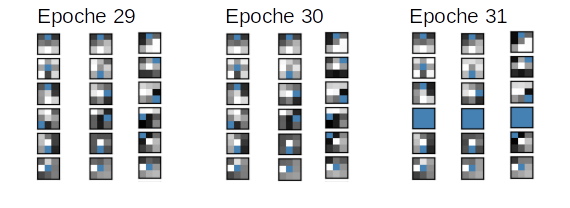
\includegraphics[width=0.9 \textwidth]{KapitelPartA/images/union.png}
 % union.png: 570x208 px, 96dpi, 15.08x5.50 cm, bb=0 0 427 156
 \caption{Beispielhafte Darstellung des Kanal-Union-Verfahrens}
 \label{abb:union}
\end{figure}



Zu diesem Zweck wird das Kanal-Union-Verfahren eingeführt. In Abbildung \ref{abb:channelUnion} wird beispielhaft ein Kanal-Union-Verfahren durchgeführt. Beim Kanal-Union-Verfahren wird eine Liste der Layer geführt, die aufeinander abgestimmt werden müssen. Im Falle eines residualen Netzes muss zusätzlich eine Liste der zusammengehörigen Layer der Kurzschlussverbindungen geführt werden. Im nächsten Schritt werden alle Eingangs- und Ausgangskanäle, die noch Gewichte größer Null haben in einer Liste gesammelt. Mit allen Elementen dieser Liste wird nun geprüft, ob mit Hilfe von Vereinigungen Kanäle gefunden werden können, die zwar keine von Null verschiedenen Gewichte mehr haben, wegen der Dimensionalität aber trotzdem beibehalten werden müssen. Alle Kanäle, die nicht unter diese Bedingung fallen, können mit Hilfe einer Rekonfiguration aus dem Netzwerk entfernt werden. In Abbildung \ref{abb:union} sind beispielhaft drei Eingangs- und sechs Ausgangskanäle dargestellt. In jedem Element des kartesischen Produkts der Menge der Eingangs- und Ausgangskanäle ist jeweils ein drei mal drei Felder großer Kernel dargestellt. Die Werte der Gewichte sind blau markiert, sobald sie absolut kleiner als der gewählte Grenzwert sind. Je dunkler die nicht-blauen Gewichte sind, desto kleiner sind sie. Da zwischen den jeweiligen Epochen für jede Batch eine Anpassung der Gewichte durchgeführt wird, entstehen teilweise große Veränderungen zwischen den Epochen. Dies ist zum Beispiel von Epoche 30 zu Epoche 31 im vierten Ausgangskanal sichtbar. Hier fällt innerhalb einer Epoche der Großteil des Ausgangskanal unter den Grenzwert.
\begin{figure}
\begin{minipage}[c]{1\linewidth}
\begin{tabularx}{1\textwidth}{m{0.2\textwidth}m{0.8\textwidth}} 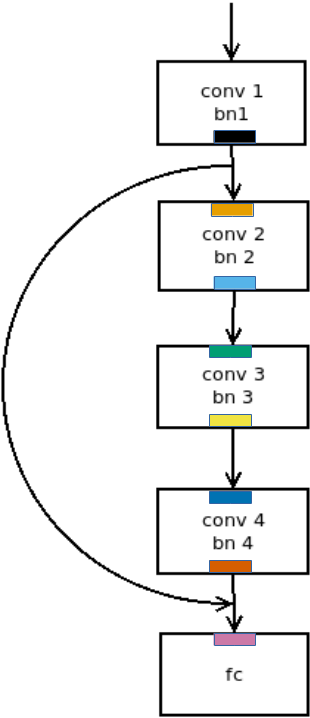
\includegraphics[width=0.21\textwidth]{KapitelPartA/images/net.png} &Liste der Layer, die direkt hintereinander sind und aufeinander abgestimmt werden müssen (ohne das zwischen den Layern eine Kurzschlussverbindung beginnt oder endet): $H=\left\{(\colorbox{sky}{2},\colorbox{bluegreen}{3}),(\colorbox{yellow}{3},\colorbox{blue2}{4}) \right\}$\newline
Liste der Layer, die im Zusammenhang mit den Kurzschlussverbindungen die gleiche Eingangskanaldimension haben müssen: \newline$E=\left\{(\colorbox{orange}{2},\colorbox{purple}{fc} \right\}$ \newline
Liste der Layer, die im Zusammenhang mit den Kurzschlussverbindungen die gleiche Ausgangskanaldimension haben müssen: $A=\left\{ ( \colorbox{black}{\textcolor{white}{1} },\colorbox{vermi}{4} ) \right\} $ \newline
Liste der dicht-besetzten Schichten vor dem ersten Beschneiden:\newline
$1:\left\{0,1,2\right\},\left\{\colorbox{black}{ \textcolor{white}{0,1,2,3,4,5,6,7}} \right\}$ \newline
$2:\left\{\colorbox{orange}{0,1,2,3,4,5,6,7}\right\},\left\{\colorbox{sky}{0,1,2,3,4,5,6,7}\right\}$\newline
$3:\left\{\colorbox{bluegreen}{0,1,2,3,4,5,6,7}\right\},\left\{\colorbox{yellow}{0,1,2,3,4,5,6,7}\right\}$\newline
$4:\left\{\colorbox{blue2}{0,1,2,3,4,5,6,7}\right\},\left\{\colorbox{vermi}{0,1,2,3,4,5,6,7}\right\}$\newline
$fc:\left\{\colorbox{purple}{0,1,2,3,4,5,6,7}\right\},\left\{0,1,2,3,4,5,6,7,8,9,10\right\}$ \newline

\\
\multicolumn{2}{m{1\linewidth}}{Liste der dicht-besetzten (db) Schichten nach dem 'auf-Null-setzen' der Parameter aber vor der Rekonfiguration:\newline
$1:\left\{0,1,2\right\},\left\{\colorbox{black}{\textcolor{white}{0,1,4,5,6,7}}\right\}$\newline
$2:\left\{\colorbox{orange}{0,1,3,5,6,7}\right\},\left\{\colorbox{sky}{0,1,2,4,5,6,7}\right\}$\newline
$3:\left\{\colorbox{bluegreen}{0,1,2,4,5,6,7}\right\},\left\{\colorbox{yellow}{0,1,2,3,5,6,7}\right\}$\newline
$4:\left\{\colorbox{blue2}{0,1,3,4,6,7}\right\},\left\{\colorbox{vermi}{0,1,3,4,5,6,7}\right\}$\newline
$fc:\left\{\colorbox{purple}{0,1,3,4,5,6}\right\},\left\{0,1,2,3,4,5,6,7,8,9,10\right\}$\newline
Vorgehen des Kanal-Union-Verfahrens:
Als erster Schritt wird für alle Elemente aus $H$ die Vereinigung von Ausgangs- und Eingangskanälen berechnet und diese dann zugewiesen:\newline
$\colorbox{sky}{2},\colorbox{bluegreen}{3}:A(\colorbox{sky}{2}) \cup E(\colorbox{bluegreen}{3})= \l\left\{\colorbox{sky}{0,1,2,4,5,6,7}\right\} \cup \left\{\colorbox{bluegreen}{0,1,2,4,5,6,7}\right\} =\left\{0,1,2,4,5,6,7\right\} $\newline
Hier wird der dünn-besetzte Kanal 3 entfernt \newline
$\colorbox{yellow}{3},\colorbox{blue2}{4}: A(\colorbox{yellow}{3}) \cup E(\colorbox{blue2}{4}) =
\left\{\colorbox{yellow}{0,1,2,3,5,6,7}\right\} \cup :\left\{\colorbox{blue2}{0,1,3,4,6,7}\right\} =\left\{0,1,2,3,4,5,6,7\right\}$\newline
Der nullwertige Eingangskanal 5 von Schicht 4 wird nicht entfernt, da der dazugehörige Ausgangskanal von Schicht 3 nicht nullwertig ist.
Im nächsten Schritt werden für die Elemente an jeweils gleicher Stelle aus den Mengen A und E Vereinigungen gebildet:
$A(\colorbox{black}{\textcolor{white}{1}})\cup A(\colorbox{vermi}{4}) \cup E(\colorbox{orange}{2}) \cup E(\colorbox{purple}{fc})=$\newline
$\left\{\colorbox{black}{\textcolor{white}{0,1,4,5,6,7}}\right\} \cup \left\{\colorbox{vermi}{0,1,3,4,5,6,7}\right\} \cup \left\{\colorbox{orange}{0,1,3,5,6,7}\right\} \cup \left\{\colorbox{purple}{0,1,3,4,5,6}\right\} = \left\{ 0,1,3,4,5,6,7\right\}$\newline
Hier wird in den Ausgangskanälen von Schicht 1 und 2 sowie in den Eingangskanälen von Schicht 2 und fc jeweils der 2. Kanal entfernt.}
\end{tabularx}
\end{minipage}
\caption{Beispielhafte Durchführung des Channel Union-Verfahrens}
\label{abb:channelUnion}
\end{figure}



Bei einem residualen Netzwerk kann weiterhin ein ganzer Block wegfallen. In diesem Fall müssen die Kanal-Union-Listen angepasst werden, die weitere Aktion wird ohne diesen Block im um mehrere Schichten verkürzten Netzwerk weiter geführt


Da mit dem Verkleinern des Netzes nicht nur potentiell Zeit sondern auch Speicherplatz gespart wird, kann bei gleicher Speicherauslastung die Batchgröße erhöht werden. Da die verwendete Technik für die Erhöhung der Batchgröße in der Quelle nicht angegeben ist und in der verwendeten Implementierung fehlt, wurde diese nachimplementiert. Dies wird in Kapitel \ref{sec:ptnew} erläutert \cite{ptImpl}. Hierbei wird die Lernrate an die erhöhte Batchgröße angepasst um negative Effekte für die Accuracy abzumildern oder auszuschließen. 

Damit lassen sich Netzverkleinerungsraten von etwa 50 \% erreichen bei weniger als 2 \% Accuracy-Verlust auf dem Datensatz Cifar10. Andere Techniken schaffen zwar zwischen 70 - 80 \% Netzverkleinerungsraten brauchen jedoch wesentlich mehr Trainingszeit \cite{lottery}. Diese großen Verkleinerungsraten sind dort sehr stark abhängig von der Initialisierung \cite{lottery}. Das heißt, nur einzelne Initialisierungen führen zu so starken Verkleinerungsraten, was insgesamt zu einer längeren Trainingszeit führt \cite{lottery}. 


Eine weitere Beschneidungstechnik arbeitet vor dem Training des Netzwerkes \cite{snyc}. Damit wird das Netz abhängig von der Initialbelegung beschnitten. Es lassen sich zwar sehr große Teile der Parameter auf Null setzen, hierbei wird im Vergleich zur Beschneidungsmethode während des Trainings allerdings weder für gemeinsames Beschneiden von Kanälen gesorgt, noch wird ein Rekonfigurationsverfahren vorgestellt. Somit hat das Netz am Ende des Verfahrens zwar relativ viele auf Null gesetzte Parameter ist aber weder schneller noch kleiner.


\section{Beschleunigung des Lernens durch Wissenstransfer}
\label{sec:net2net}
Beim Trainieren eines CNNs kommt es häufig vor, dass nach initialem Wählen der Tiefe beziehungsweise Breite des Netzes diese Parameter in einem weiteren Trainingslauf erhöht werden und in Folge dessen das Netzwerk komplett neu trainiert werden muss. Mit Hilfe der Quelle zu diesem Unterkapitel wurde ein Verfahren geschaffen, welches das Netz tiefer oder breiter machen kann und dabei die im ersten Trainingsdurchlauf trainierten Gewichte weiter verwendet \cite{net2net}. Durch diesen Wissenstransfer von einem Netz zu einem tieferen oder breiteren Netz wird eine schnellere Konvergenz des neuen Netzes erwartet. Durch die Initialisierung mit schon vorhandenen Parametern entsteht eine Transformation, die die erlernte Funktion erhält.

\begin{figure}[h]
 \centering
 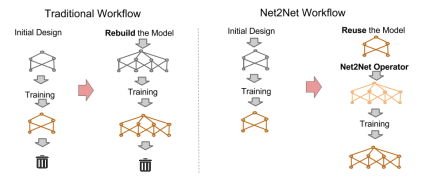
\includegraphics[width=0.7\textwidth]{KapitelPartA/images/net2net.png}
 % net2net.png: 433x179 px, 72dpi, 15.28x6.31 cm, bb=0 0 433 179
 \caption{Traditioneller Workflow vs. Net2Net Workflow}
 \label{abb:net2net}
\end{figure}


Wie in Abbildung \ref{abb:net2net} abgebildet ist, lässt sich so der Arbeitsablauf zum Finden der passenden Netzstruktur anders gestalten. Der Net2Net-Operator macht hier das Netz entweder breiter (mehr Kanäle in bestimmten Schichten) oder tiefer (zusätzliche Schichten). Diese beiden Operatoren werden nun vorgestellt.

\subsubsection{Operator für breiteres Netz}
Beim Operator für ein breiteres Netz werden für eine bestimmte Schicht Ausgangskanäle und für die nachfolgende Schicht Eingangskanäle hinzugefügt. Die Schicht, der die Ausgangskanäle hinzugefügt werden, wird mit $j$ bezeichnet und hat den Gewichtstensor $\mathbf{W}_j$ mit der Dimensionalität von $n \times l \times d(h_{l,1}) \times d(h_{l,2}$. Die Schicht, der die Eingangskanäle hinzugefügt werden wird mit $j+1$ bezeichnet und hat den Gewichtstensor $\mathbf{W}_{j+1}$ mit der Dimensionalität von $m \times n \times d(h_{j+1,1}) \times d(h_{j+1,2})$. Dem Layer $j$ werden $q$ Kanäle hinzugefügt. Dies entspricht wie in Abbildung \ref{abb:channels} abgebildet ist $q \cdot l $ zusätzlichen Kerneln. 
\begin{figure}[h]
 \centering
 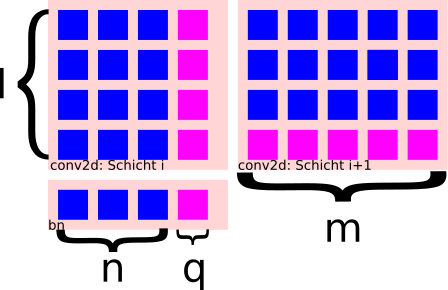
\includegraphics[width=0.6\textwidth]{KapitelPartA/images/channels.png}
 % channels.pdf: 0x0 px, 300dpi, 0.00x0.00 cm, bb=
 \caption{Übersicht über die zusätzlichen Kanäle}
\label{abb:channels}
 \end{figure}



Für den Layer $j+1$ sind es entsprechend $q \cdot m $ zusätzliche Kernel. Die Gewichtstensoren nach dem Anwenden des Net2Net-Operators werden mit $\mathbf{U}^j$ und $\mathbf{U}^{j+1}$ bezeichnet und sollen die Dimensionalität von $\mathbf{U}^j: (n+q) \times l \times d(h_{(j,1)}) \times d(h_{(j,2)})$ und $\mathbf{U}^{j+1}: m \times (n+q) \times d(h_{(j+1,1)}) \times d(h_{(j+1,2)})$ haben. Der Net2Net-Operator wird angewendet, indem zunächst eine Mapping-Funktion $g$ definiert wird, die für eine zufällige Belegung der zusätzlichen Kernels sorgt:

\begin{equation}
 g(j) =  
 \begin{cases}
 j & , \text{ falls} \, j \leq n \\
 k & , \text{ falls} \, j>n : \;  k \text{ zufälliges Sample von} \left\{ 1,2,\ldots, n \right\} \\ 
 \end{cases} 
 \end{equation}
 Mit Hilfe dieser Mapping-Funktion werden nun die neuen Gewichtstensoren initialisiert:
 \begin{align*}
 \mathbf{U}_j(e,f,h_{j,1},h_{j,2}) &= \mathbf{W}_j(g(e),f,h_{j,1},h_{j,2}) \\
 \mathbf{U}_{j+1}(e,f,h_{j+1,1},h_{j+1,2})&= \frac{1}{|\left\{ x | g(x)=g(a)\right\}|}\mathbf{W}_{j+1}(e,g(f),h_{j+1,1},h_{j+1,2})
 \end{align*}
Die Funktion $g(j)$ wird dabei für jede neu hinzugekommene Schicht nur einmal ausgewertet, sodass gesamte Reihen statt einzelner Kernel kopiert werden. Sollte sich zwischen dem $j$-ten und $(j+1)$-Layer eine Batchnormalisierungsschicht befinden, so werden die Parameter dieser Schicht ebenfalls kopiert.

Um nicht mehrere exakt gleiche Kernelreihen zu haben kann außerdem noch ein Noiseanteil auf alle Gewichte addiert werden. Dies ist vor allem für den Fall wichtig, wenn der Trainingsalgorithmus keine Form der Randomisierung hat, das heißt die gleichen Gewichtstensoren werden ermutigt, unterschiedliche Funktionen zu erlernen. Somit sind die vom ursprünglichen und neuen Netz gelernten Funktionen ähnlich aber nicht gleich.

\subsubsection{Tieferes Netz}

Der Operator für ein tieferes Netz ersetzt die Operation der $j$-ten Schicht $\mathbf{v}_{i,j} = \text{BN}_{\gamma,\beta}( \mathbf{v}_{i,j}* \mathbf{W}_{j})$ durch die Operation von zwei Layern  
\begin{equation}
\mathbf{v}_{i,j} =\text{BN}_{\gamma',\beta'}( \text{BN}_{\gamma,\beta}( \mathbf{v}_{i,j} * t(W_{j})) * t(U_{j})    )
\end{equation}
$\mathbf{U}$ wird als Identitätsmatrix initialisiert.
Da zwischen den beiden Layern eine Batchnormalisierung genutzt wird, müssen die Parameter der Batchnormalisierung $\gamma'$ und $\beta'$ so gewählt werden, dass sie die gelernte Funktion des Netzes nicht verändern.


\subsubsection{Diskussion der Methode}

Die beiden Net2Net-Operatoren schaffen die Möglichkeit, Familien von Netzarchitekturen zu erforschen ohne jedes Mal von neuem zu lernen. Mit Hilfe der beiden Operatoren lässt sich die Komplexität des Netzes erhöhen ohne die gelernte bisherige Funktion zu vernachlässigen.




\section{Automatische Architektursuche}\label{sec:auto}
Neben dem im letzten Kapitel ausführlich erläuterten Ansatz des Strukturlernens gibt es noch einige andere aktuelle Ansätze, die automatisch nach einer besseren Architektur für einen Datensatz suchen. Einige dieser Ansätze werden hier beleuchtet und es wird gezeigt, wieso das im letzten Kapitel erläuterte Verfahren im praktischen Teil weiter verwendet wird.

Beim Versuch die Hyperparameter eines Netzes sinnvoll automatisch zu wählen, entsteht ein sehr großer Suchraum. Dieser Suchraum lässt sich mit viel Aufwand absuchen \cite{dvolver}. Es entsteht ein Optimierungsproblem mit mehreren zu optimierenden Variablen bei welchem eine Pareto-Front gesucht wird \cite{dvolver}. Das Ergebnis schafft eine Verbesserung der Accuracy gegenüber bekannten Architekturen, dabei summiert sich allerdings die Trainingszeit mit 20 NVIDIA V100 Grafikkarten für Imagenet auf 2,5 Tage\cite{dvolver}.
Eine weitere Methode den Suchraum zu durchsuchen sind genetisch inspirierte Suchalgorithmen \cite{gen}. Dabei wird initial eine Population von Netzen gebildet \cite{gen}. Nach einem Trainingsdurchgang werden diese nach ihrer Fitness (Klassifikationsleistung) selektiert \cite{gen}. Im weiteren Verlauf werden jeweils zwei dieser Netze gepaart und es entsteht eine neue Generation an Netzen \cite{gen}. Allerdings ist hier die Trainingszeit in einem Rahmen von 35 GPUs für einen Tag \cite{gen}. Dann ist die Architektursuche allerdings komplett automatisiert und erreicht eine Accuracy von 96.78 \% für Cifar 10 und 79.77 \% für Cifar 100 \cite{gen}. \footnote{Um diese Zahl einordnen zu können: die besten zehn Accuracy-Werte liegen für Cifar 10 bei 96.62 \% bis 99.37 \% und für Cifar 100 bei 82,35 \% bis 93,51 \%. Entsprechende Veröffentlichungen sind unter \url{https://benchmarks.ai/} zu finden}  

Das Ziel von einigen Veröffentlichungen im Themenbereich der automatischen Architektursuche ist es, diese lange Trainingszeit zu reduzieren.

Eine Möglichkeit der Reduzierung bietet sich durch Ausnutzung von domainspezifischen Eigenschaften der zu klassifizierenden Bilder. Eine Möglichkeit einer domainspezifischen Eigenschaft, die genutzt werden kann, ist, wenn die Bilder nicht klassisch mit einer Kamera, sondern mit anderen Geräten aufgenommen wurden. Diese veränderte Aufnahmeart kann dafür sorgen, dass sich der Suchraum massiv einschränken lässt und sich damit die Architektursuche beschleunigt.
Als Beispiel kann hier eine Radaranlage zur Aufnahme von Bilder dienen \cite{polsar}.


Eine weitere Möglichkeit die Trainingszeit zu minimieren ist es, den Suchraum deutlich zu verkleinern und die Anzahl an Durchläufen zu minimieren. Der Nachteil ist dann allerdings, dass die Wahrscheinlichkeit, ein Netz in einem globalen Optimum zu finden bezüglich des Suchraumes klein ist. Eine Methode die dies nutzt, wird im nächsten Unterkapitel vorgestellt.

\section{Schnelles Ressourcen-beschränktes Strukturlernen tiefer Netzwerke}\label{sec:morphnet}
Im Gegensatz zu den Kapiteln \ref{sec:prunetrain} und \ref{sec:net2net}, in denen jeweils eine Möglichkeit, ein CNN kleiner sowie größer zu machen vorgestellt wurden, geht es jetzt darum, dies zu kombinieren. Die Quelle für diese Kapitel ist, soweit nicht anders gekennzeichnet, das Paper, welches die Methode vorgestellt hat.

Die manuelle Wahl von Hyperparametern, die bestimmen wie groß und komplex ein neuronales Netz ist, 
braucht Erfahrung und Kunstfertigkeit. Sind die Hyperparameter falsch gewählt, so müssen diese angepasst und das Netz erneut trainiert werden. Mit Hilfe der hier vorgestellten Methode wird die Suche nach der besten Architektur automatisiert. Dies geschieht mit Hilfe von iterativen Verkleinern und Vergrößern des Netzes. Diese Methode hat drei Vorteile:
\begin{enumerate}
 \item Es ist auf große Netze und große Datensätze skalierbar
 \item Es kann die Struktur in Bezug auf eine bestimmte Nebenbedingung (zum Beispiel Modellgröße, Anzahl an Parametern) optimieren
 \item Es kann eine Struktur lernen, die die Performance erhöht
\end{enumerate}

Das Ziel der Methode ist es, automatisch die beste Architektur für ein Netz zu finden. Dies umfasst die Breiten der Eingangs- und Ausgangskanäle, Größe der Kernel, die Anzahl der Schichten und die Konnektivität dieser Schichten. Im Rahmen dieser Methode wird dies auf die Breite der Ausgangskanäle eingeschränkt. Die Methode kann auf die anderen Größen erweitert werden. Allerdings ist die Einschränkung auf die Breite der Ausgangskanäle sowohl effektiv als auch simpel.
Die Breite der Ausgangskanäle für alle $J$ Schichten wird mit $\mathcal{C}_{1:J}$ bezeichnet. 

Der Anfangspunkt dieser Methode ist ein Netz $\mathcal{W}^1$ mit einer initialen Breite der Ausgangskanäle sowie fixen Filtergrößen. Die Nebenbedingung wird mit der Funktion $\mathcal{F}$ bezeichnet. Sie optimiert entweder die Modellgröße oder die Anzahl an Flops per Inferenz. Die Methode optimiert formal gesehen also folgendes:
\begin{equation}
 \mathcal{W}^{\ast}= \underset{\mathcal{F}(\mathcal{C}_{1:J})\leq \zeta}{\text{arg min}} \underset{\mathcal{W},\mathbf{x}_i \in \mathcal{B}}{\text{ min}}\; l(f(\mathbf{x_i}, \mathcal{W}),y_i)\label{equ:morph1}
\end{equation}

Das Vergrößern des Netzes basiert auf einer Lösung für die Gleichung \ref{equ:morph1}: dem Breitenmultiplikator $\omega$. 
Sei $\omega \cdot O_{1:M} = \left\{ \lfloor \omega O_1 \rfloor, \lfloor \omega O_2 \rfloor, \ldots , \lfloor \omega O_M \rfloor \right\}, \omega>0$. Gilt $\omega>1$, so wird das Netz vergrößert. Bei $\omega <1$ wird das Netz verkleinert. Um die Gleichung \ref{equ:morph1} zu lösen, finde nun das größte $\omega$, so dass $\mathcal{F}(\omega \cdot O_{1:M})\leq \zeta$ gilt.


Dieser Ansatz sorgt für eine mögliche Verkleinerung und Vergrößerung des Netzes und er funktioniert gut bei einem guten initialen Netz. Ist das initialen Netz aber nicht von so guter Qualität, so hat dieser Ansatz Probleme. Grund hierfür ist wahrscheinlich ein lokales Minimum, aus welchem die Optimierungsfunktion nicht mehr herausfindet, um ein besseres lokales oder globales Minimum zu finden.

Dieser Nachteil wird durch eine Veränderung der Verlust-Funktion aufgehoben. Es wird ein Regularisierer $\mathcal{G}$ dazu addiert, welcher misst, wie groß der Anteil eines Netzbestandteiles an $\mathcal{F}( \mathcal{C}_{1:J})$ ist, und der es damit direkt optimieren kann. Dann ist
\begin{equation}
 W^{\ast}= \underset{\mathcal{F}(\mathcal{C}_{1:J})\leq \zeta}{\text{arg min}} \underset{\mathcal{W}}{\text{min}}\; l(f(\mathbf{x_i}, \mathcal{W}),y_i) + \lambda \mathcal{G}( \mathcal{W})  
 \label{equ:morph2}
\end{equation}
Dieser Ansatz kann die relative Größe einer Schicht ändern, hat aber den Nachteil das häufiger die zu optimierende Nebenbedingung nicht optimal maximiert wird.


Die beiden Ansätze lassen sich kombinieren. Algorithmus \ref{alg:morphnet} beschreibt den Algorithmus der bei der Kombination entsteht mit Pseudocode.
\begin{algorithm}[H]
\caption{MorphNet Algorithmus}
\begin{algorithmic}[1]
\STATE Trainiere das Netz um $\mathcal{W}^{\ast}=\underset{\mathcal{W}}{arg min}\; l(f(\mathbf{x_i}, \mathcal{W},y_i) + \lambda \mathcal{G}(\mathcal{W}))$ zu finden
\STATE Finde die neue Breite $\mathcal{C}_{1:J}^{\prime}$, die durch 1. errechnet wurde
\STATE Finde das größte $\omega$, so dass $\mathcal{F}(\omega \cdot \mathcal{C}_{1:J})\leq \zeta$ gilt
\STATE Wiederhole ab 1. so häufig wie gewünscht mit $\mathcal{C}_{1:J} = \mathcal{C}_{1:J}^{\prime}$
\ENSURE $\omega \cdot \mathcal{C}_{1:J}$
\end{algorithmic}
\label{alg:morphnet}
\end{algorithm}
Dieser Algorithmus kann so oft durchlaufen werden bis entweder die Performance des Netzes gut genug ist, oder bis die letzten Durchläufe keine Veränderungen mehr hervorgebracht haben.


\subsection{Definition der Nebenbedingung}
Die Nebenbedingung $\mathcal{F}$ lässt sich für verschiedene zu optimierende Zielgrößen definieren. Eine einfache Nebenbedingungen, die Modellgröße wird hier beispielhaft erläutert. Die Größe dieser Nebenbedingung wird vor allem durch Schichten mit Matrixmultiplikation dominiert. Die Modellgröße ergibt sich durch die Größe der Tensoren der einzelnen Schichten. Da die Größe der Tensoren der einzelnen Schichten abhängig von der Anzahl der Eingangs- und Ausgangskanäle sowie der Filtergröße und nicht von der Position im Netzwerk ist, lässt sich $\mathcal{F}(\mathcal{C}_{1:J})$ auf die einzelnen Schichten zurückführen. Es gilt:
\begin{equation}
 \mathcal{F}(\mathcal{C}_{1:J})=\sum_{j=1}^{J} \mathcal{F}(j)
\end{equation}
Für den Breitenmultiplikator $\omega$ gilt: $\mathcal{F}(\omega \cdot \mathcal{C}_{1:J}=\sum_{j=1}^{J} \omega \cdot \mathcal{F}(j)$

Die Abhängigkeit von der Größe des jeweiligen Tensors ergibt für 
\begin{equation}\label{equ:F}
\mathcal{F}(j)=c_j \cdot k_j \cdot d(h_{j,1}) \cdot d(h_{j,2})  
\end{equation}
Da durch die Anwendung des Regularisierers einzelne Kanäle auf Null gesetzt werden und ein Netz ohne diesen Kanal möglich wäre, sollen diese Kanäle in dieser Berechnung ausgelassen werden. Daher wird die Formel um Aktivierungsfunktionen $A_{k_l,j}$ und $B_{c_l,j}$ ergänzt die mit einer Eins angeben, dass der zugehörige Kanal nicht null ist. Eine Null als Ergebnis der Aktivierungsfunktion ergibt sich, wenn der entsprechende Kanal komplett auf Null gesetzt wurde. Dadurch lassen sich $c_j$ und $k_j $ aus Formel \ref{equ:F} ersetzen:
\begin{equation}
\mathcal{F}(j)=\left(\sum_{k=1}^{k_l} A_{k,j} \right) \cdot \left(\sum_{c=1}^{c_l} B_{c,j}\right) \cdot d(h_{j,1}) \cdot d(h_{j,2})  
\end{equation}


\subsection{Regularisierer}
Beim Verkleinern des Netzes soll die Verlustfunktion $l$ des CNN mit der Nebenbedingung $\mathcal{F}(\mathcal{C}_{1:J})\leq \zeta$ minimiert werden. Bei der Wahl des Regularisierers muss bedacht werden, dass der Regularisierer und seine Ableitung kontinuierlich definiert sein müssen, da die Parameter im Netz durch ein Gradientenabstiegsverfahren gelernt werden. Zusätzlich kann eine Nebenbedingung nicht direkt durch ein Gradientenabstiegsverfahren gelernt werden. Daher wird $\mathcal{F}$ in veränderter Form als Regulariser gewählt. Die Veränderung umfasst das Hinzufügen von $\gamma$, die ähnlich einer Batchnormalisierung genutzt werden:
\begin{equation}
\mathcal{G}(j)=\left(\sum_{k=1}^{k_l-1} A_{k_l,j} \sum_{c=1}^{c_l-1} |\gamma_{c, j} | \right) \cdot \left(\sum_{k=1}^{k_l-1} |\gamma_{k,j} |   \sum_{c=1}^{c_l-1} B_{c,j}\right) \cdot d(h_{j,1}) \cdot d(h_{j,2})  
\end{equation}

Mit dieser Funktion lässt sich mittels Gradientenabstieg lernen, obwohl Teile des Regularisieres nicht komplett kontinuierlich sind. $\gamma$ muss dabei kontinuierlich sein. Werden die $\gamma$ für einen Kanal auf Null gesetzt durch das Lernen, so ist der dazugehörige Kanal aus der Berechnung wie gewünscht ausgeschlossen. Für jeden Ein- und Ausgangskanal einer Schicht wird ein $\gamma$ in den Vorwärts-Durchgang eingebaut. Diese Parameter funktionieren dann analog zu den $\gamma$ aus der Batchnormalisierung, da sie kontrollieren, welcher Prozentsatz eines Kanals weitergeleitet wird.


Aus dem Regularisierer einer Schicht lässt sich mittels Addition die Regularisierung des kompletten Netzes berechnen.
\begin{equation}
 \mathcal{G}(\mathcal{W})=\sum_{j=1}^{J} \mathcal{G}(j)
\end{equation}


Um die Wichtigkeit vom besseren Training des Netzes und der Regularisierung von Parametern treffen zu können wird ein Parameter $\lambda$ eingeführt. So entsteht die Verlust-Funktion
\begin{equation}
 \mathcal{W}^{\ast}=\underset{\mathcal{W}}{arg min}\; \; l(f(\mathbf{x}_i, \mathcal{W}),y_i) + \lambda \mathcal{G}(\mathcal{W})
\end{equation}



Dieser Regularisierer funktioniert nicht für Netze, die Kurzschlussverbindungen besitzen. Hier wird, wie beim Beschneiden des Netzes während des Trainings, ein Gruppen-Lasso verwendet. Dies stellt sicher, dass an Kurzschlussverbindungen nur so beschnitten werden kann, wie es für die Dimensionalität des Netzes zuträglich ist.







\section{Verringerung der für Berechnungen nötige Zeit}

Die Zeit, die ein Convolutional Layer braucht um berechnet zu werden hängt ab von:
\todo{Fehlt hier noch etwas?}
\begin{itemize}
 \item der Filtergr\"osse
 \item der Bildgr\"osse
 \item dem verwendeten Zahlenformat
\end{itemize}
Beim Verändern der Filter- oder der Bildgr\"osse, um Trainingszeit zu sparen, ver\"andert sich auch die Erkennungsleistung \todo{cite}. Dies ist beim Verändern des verwendeten Zahlenformats nicht umbedingt gegeben. Standardformat ist eine 32 Bit Gleitkommazahl. Die einfachste Methode hier Trainingszeit zu sparen ist das Halbieren der Bitanzahl auf 16 Bit. Eine weitere Methode ist das Benutzen von 16 Bit Dynamischen Festkommazahlen.
Die beiden alternativen Methoden haben unterschiedliche Anforderungen an die Ausführungsplattform. Diese Anforderungen und die Besonderheiten der beiden Verfahren werden in den folgenden zwei Unterkapiteln näher beleuchtet.


\subsection{Berechnung mit 16 Bit Gleitkomma}

Die 16 Bit Gleitkommazahl unterscheidet sich nicht nur in der Länge von der 32 Bit Zahl sondern aus der unterschiedlichen Länge erwachsen Unterschiede in den darstellbaren Zahlen. In Tabelle \todo{ref} sind diese Unterschiede dargestellt.





Diese Nachteile von 16 Bit Gleitkommazahlen können durch drei Techniken abgemeildert oder sogar komplett aufgehoben werden:
\begin{itemize}
 \item 32 Bit Mastergewichte und Updates
 \item Sklaierung der Loss-Funktion
 \item Arithmetische Präzision 
\end{itemize}

Diese drei Techniken werden in den drei folgenden Unterkpaiteln behandelt.

\subsubsection{32 Bit Mastergewichte und Updates}

Beim Trainieren von neuronalen Netzwerken mit 16 Bit Gleitkommazahlen werden die Gewichte, Aktivierungen und Gradienten im 16 Bit Format gespeichert. Die Speicherung der Gewichte als 32 Bit Mastergewichte hat zwei mögliche Erklärungen, die aber nicht immer zutreffen müssen. 

Um nach einem Forward Druchlauf des Netzes die Gewichte abzudaten wird ein Gradientenabstiegsverfahren benutzt. Hierbei werden die Gradienten der Gewichte berechnet. Um für die Funktion, die das CNN approximiert einen besseren Approximationserfolg zu erlangen wird dann dieser Gradient mit der Lernrate multipliziert. Wird dieses Produkt in 16 Bit abgespeichert, so ist in viele Fällen das Produkt der beiden Zahlen gleich Null. Dies liegt an der Taqtsache, dass wie in Tabelle \todo{ref} zu sehen ist die kleinste darstellbare Zahl in 16 Bit wesentlich grösser ist als in 32 Bit.


Der zweite Grund wieso man Mastergewichte brauchen könnte ist die Tatsache, dass bei grossen Gewichten die Länge der Mantisse nicht ausreicht, um sowohl das Gewicht als auch das zu  addierende Update zu speichern.

Aus den beiden Gründen wird das in Abbildung \todo{ref} gezeigte Schema zum Trainieren einer Schicht mit gemischt präzisen Gleitkommazahlen benutzt.

\missingfigure{Schema}

\subsubsection{Sklaierung der Loss-Funktion}

\subsubsection{Arithmetische Präzision}


\subsection{Berechnung mit 16 Bit Dynamischen Festkommazahlen}


Quelle: \cite{FPGpu}


\subsection{Beschleunigung der Berechnung des Gradientenabstiegsverfahren}
\todo[inline]{Überblick schreiben; 4 Stunden}
Bei der Beschleunigung der Berechnung des Gradientenabstiegsverfahren gibt es vier verschiedene publizierte Herangehensweisen:
\begin{itemize}
 \item Accelerating CNN Training by Sparsifying Activation Gradients
 \item Weight Normalization: A Simple Reparameterization
to Accelerate Training of Deep Neural Networks
 \item Accelerating Deep Neural Network Training with Inconsistent Stochastic Gradient Descent
 \item Accelerated CNN Training Through Gradient Approximation 
\end{itemize}


\subsubsection{Accelerating CNN Training by Sparsifying Activation Gradients}

\subsubsection{Weight Normalization: A Simple Reparameterization
to Accelerate Training of Deep Neural Networks}




\subsubsection{Accelerating Deep Neural Network Training with Inconsistent Stochastic Gradient Descent}



\subsubsection{Accelerated CNN Training Through Gradient Approximation }




\section{Additive Methoden}
Die Methoden in diesem Kapitel beeinflussen die Trainingszeit nicht direkt, sondern helfen die Folgen anderer Verfahren abzumildern.

\subsection{Ghost Batch Normalization}





\cleardoublepage
\chapter{Einleitung}
\label{sec:EinleitungGesamt}

\section{Motivation und Hintergrund dieser Arbeit}


MorphNet ist eine Möglichkeit mittels Verkleinern und Vergrössern des Netzwerkes effizient die Struktur eines Netzwerks zu lernen. Ist dieses Konzept auch auf PruneTrain zu übertragen und so zu erweitern, dass nicht das komplette Netz erweitert wird, sondern eben nur sinnvolle Bereiche?
Ist dieser Prozess mit Hilfe weiterer Methoden beschleunigbar?

\todo[inline]{Einleitung fertigschreiben -- zum Schluss}

\section{Aufbau der Arbeit}
\todo[inline]{Aufbau der Arbeit -- erst bei fortgeschrittener Arbeit schreiben}


\section{Suchbegriffe}
\todo[inline]{verwendete Suchbegriffe}


\section{Experimentales Setup}


\subsection{Hardware}
Server mit 4 Graka:

2 mal Geforce GTX 1080 Ti mit CUDA Version 10.1 

2 mal Geforce RTX 2080 Ti mit CUDA Version 10.1

\subsection{Wahl des Frameworks}

Es wird mit pytorch gearbeitet, da pytorch gegenüber anderen Frameworks eine grössere Flexibiltät erlaubt. Ausserdem ist eine fast vollständige Implementierung von PruneTrain in Pytorch geschrieben. Diese wird im nächsten Kapitel untersucht und soweit erweitert, dass es dem Stand im PruneTrain Paper entspricht.

Pytorch bietet mit cudnn und cuda im Hintergrund gute Möglichkeiten die Trainingszeiten einzelner Epochen zu messen und sie so mit einander zu vergleichen.


\subsection{verwendete Netzarchitektur}\label{sec:archi}
Die PruneTrain Implementierung hat initial mehrere verschiedene Netzarchitekturen zur Auswahl:
\begin{itemize}
 \item AlexNet
 \item ResNet 32/50
 \item vgg 8/11/13/16
 \item mobilenet
\end{itemize}

Schränke diese Auswahl auf ResNet ein.
Gründe hierfür:
\begin{itemize}
 \item Da die Überlegung besteht diese Netze tiefer zu machen wähle ResNet, da die Identity-Übergänge dem Netz erlauben das degradation Problem zu umgehen während das Netz noch tiefer/ breiter wird.
 \item Festlegung auf eine Architektur um Umfang der Arbeit zu begrenzen
\end{itemize}

Erweitere dies jedoch durch beliebige grosse ResNets. Ein ResNet ist hier durch 4 Parameter charaterisiert:

\begin{itemize}
 \item $s$: Anzahl an Stages, die das ResNet hat
 \item $[n]:$ Anzahl von Blöcken pro Stage 
 \item $l$: Anzahl von (Conv+Batch)-Layer pro Block
 \item $b$: Boolean Parameter, der angibt ob die Blöcke im Netz die Bootleneck-Eigenschaft haben
\end{itemize}
\todo[inline]{Bottleneck -Eigenschaft}
\subsection{Überblick über das experimentelle Vorgehen}


\section{Untersuchung von PruneTrain}

Die Untersuchung von PruneTrain basiert auf einer bereits vorgefertigten Implementierung \cite{ptImpl}. 

\subsection{Evaluation von PruneTrain}

Hier wird das Ergebnis der Ausführung von PruneTrain auf der Hardware mit den Ergebnissen aus dem Prune Train Paper verglichen. Im ersten Abschnitt wird zunächst betrachtet, wie sich die Trainingszeiten bei den veränderbaren Hyperparametern von PruneTrain verändern. Im zweiten Abschnitt wird betrachtet, wie sich die Accuracy im Verlauf der Epochen verhält.

Als Netzwerk wird ein Res-Net 32 verwendet. In Tabelle \todo{ref} ist die Netzstruktur aufgeführt.



verwendete Kenngrößen:

\begin{itemize}
 \item 1 GPU
 \item Cifar10
 \item 180 Epochen
\end{itemize}

Zunächst wird hierfür nur das Prune Train ohne Anpassung der Batchgrösse betrachtet. 

Variable Größen, die in verschiedenen Experimenten geändert werden:

\begin{itemize}
 \item Lernrate
 \begin{itemize}
  \item unterschiedlich große Lernraten
  \item Anpassung der Lernrate währenddem Training
 \end{itemize}

 \item Rekonfigurationsinterval
 \item Threshold
 \item Lasso-Ratio
 \item Batchgröße:
 \begin{itemize}
  \item unterschiedliche Batchgrößen verschiedener Durchläufen
  \item Anpassung der Batchgröße währenddem Training
 \end{itemize}
\end{itemize}

Um die Experimente mit den unterschiedlich großen Kenngrößen vergleichen zu können wird jeweils eine Größe geändert und der Einfluss dieser Größe auf die Trainingszeit betrachtet. Betrachte zunächst eine feste Batchgröße von 256 über alle 180 Epochen und vergleiche diese mit mehreren Durchläufen des Baseline-Netzes. 
\subsubsection{Experimente zur Lernrate}

Die Trainingszeiten in Sekunden pro Epoche für verschiedene Lernrate ist in Abbildung \ref{abb:lr} zu sehen. Unterschiede zwischen den Experimente sind in Abbildung \ref{abb:lr1} zunächst nicht direkt sichtbar. Um diese besser sichtbar zu machen wird für jedes Experimente die Summeder Trainingszeiten über die Epochen gebildet. In Abbildung \ref{abb:lr2} ist zu beobachten, dass beim größten Threshold die geringste summierte Trainingszeit zusammenkommt. Da bei einem höheren Threshold im Laufe des Trainings mehr Gewichte unter den Grenzwert fallen und somit entfernt werden. Liegen diese Gewichte sinnvoll, so können ganze Kanäle entfernt werden.
 \begin{figure}[h]
 \centering
 \subfloat[][verschiedene Experimente]{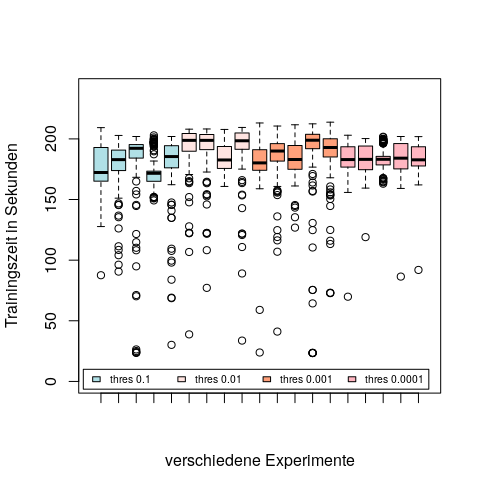
\includegraphics[width=0.37\textwidth]{KapitelPartB/Images/thres1.png}\label{abb:lr1}}
 \qquad
 \subfloat[][Summe verschiedener Experimentengruppen]{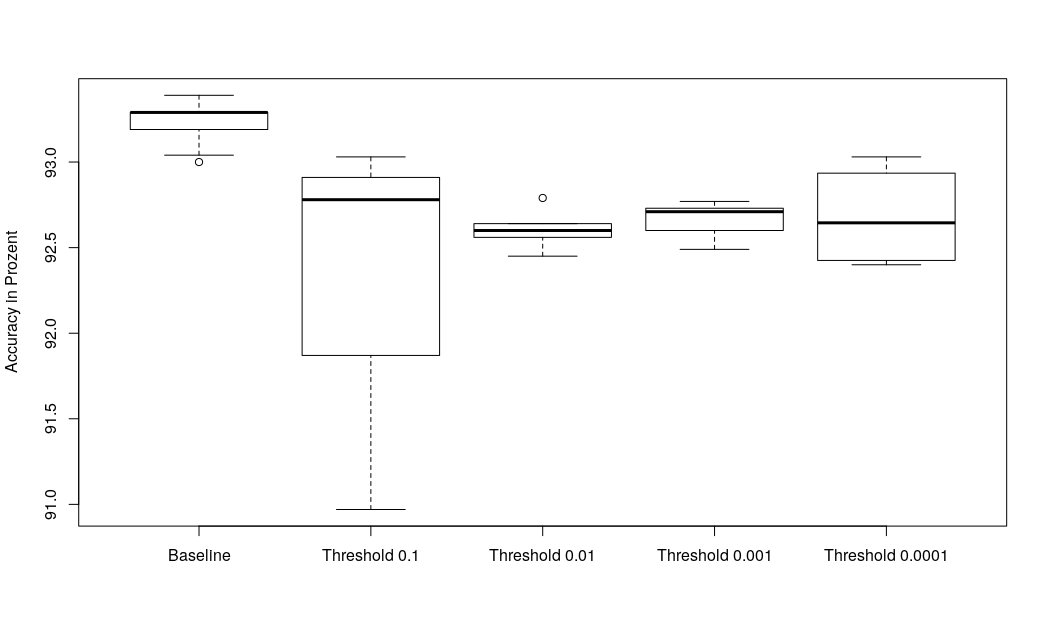
\includegraphics[width=0.55\textwidth]{KapitelPartB/Images/thres2.png}\label{abb:lr2}}
 \caption{Boxplot der verschiedenen Grenzwerte}
 \label{abb:lr}
\end{figure}
 
 In Abbildung \ref{abb:lr3} ist zu sehen, dass der gleiche Effekt sich auch bei Accuracy zeigt. Die Accuracy für den größten Grenzwert ist am niedrigsten.
 
 \begin{figure}[h]
 \centering
 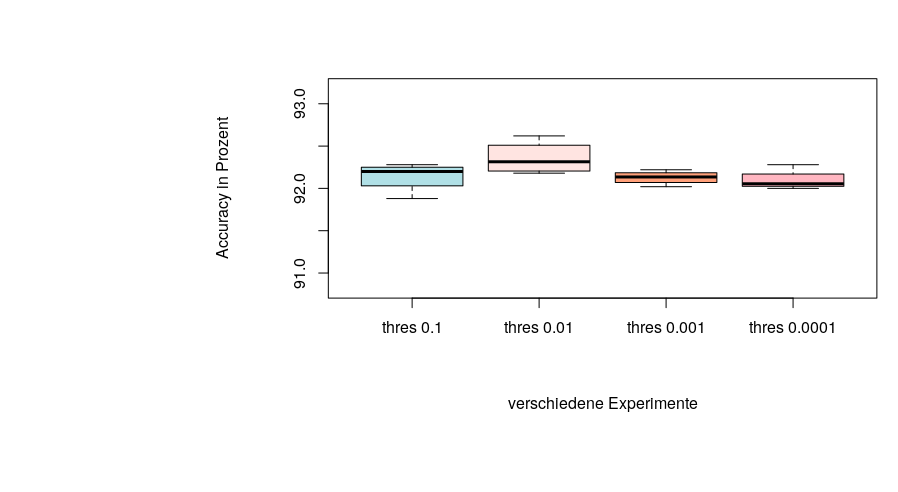
\includegraphics[width=0.8\textwidth]{KapitelPartB/Images/thres3.png}
 % reconf3.png: 454x491 px, 96dpi, 12.01x12.99 cm, bb=0 0 341 368
 \caption{Accuracy von verschiedenen Experimentengruppen des Grenzwerts}
 \label{abb:lr3}
 \end{figure}


\subsubsection{Experimente zum Rekonfigurationsintervall}

 Als nächste Größe wird der Einfluss des Rekonfigurationsintervalls überprüft. Die entsprechenden Grafiken sind in Abbildung \ref{abb:reconf} abgebildet. In Abbildung \ref{abb:reconf1} sind für die verschiedenen Experimente die Trainingszeiten pro Epoche zu sehen. Dabei werden drei verschiedene Rekonfigurationsintervalle (2,5 und 10) verglichen. In Abbildung \ref{abb:reconf1} lässt sich für die verschiedenen Experimente keine großen Unterschiede sehen. Werden die Zeiten der jeweiligen Experimente addiert und in einem Boxplot dargestellt entsteht Abbildung \ref{abb:reconf2}. In dieser Abbildung ist deutlich zu sehen, dass mit steigendem Rekonfigurationsintervall auch die Summe der Trainingszeiten pro Epoche steigt.
 
 \begin{figure}[h]
 \centering
 \subfloat[][verschiedene Experimente]{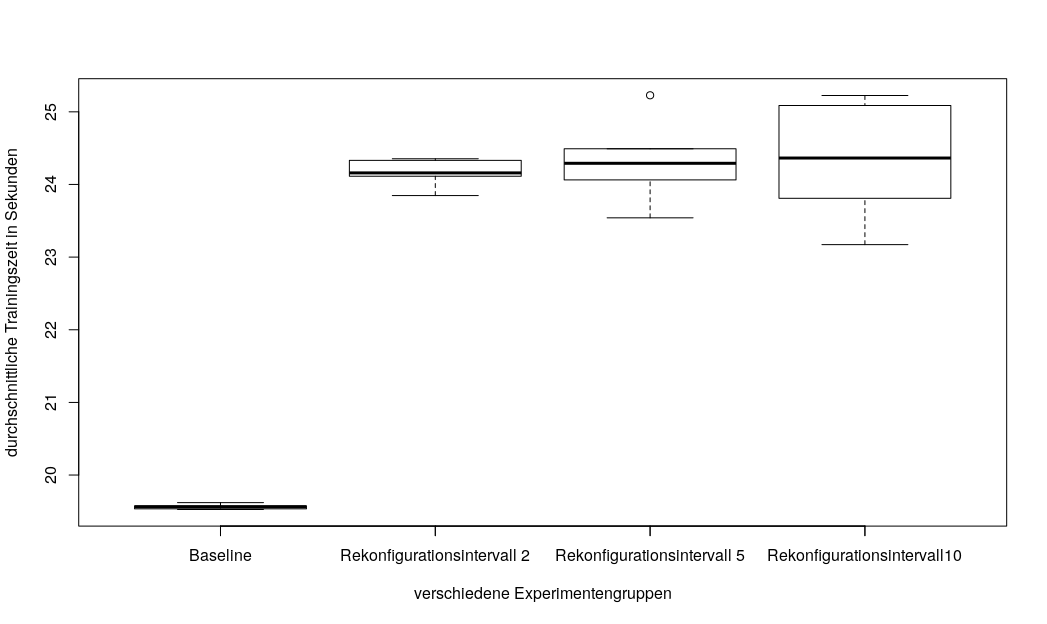
\includegraphics[width=0.47\textwidth]{KapitelPartB/Images/reconf1.png}\label{abb:reconf1}}
 \qquad
 \subfloat[][Summe verschiedener Experimentengruppen]{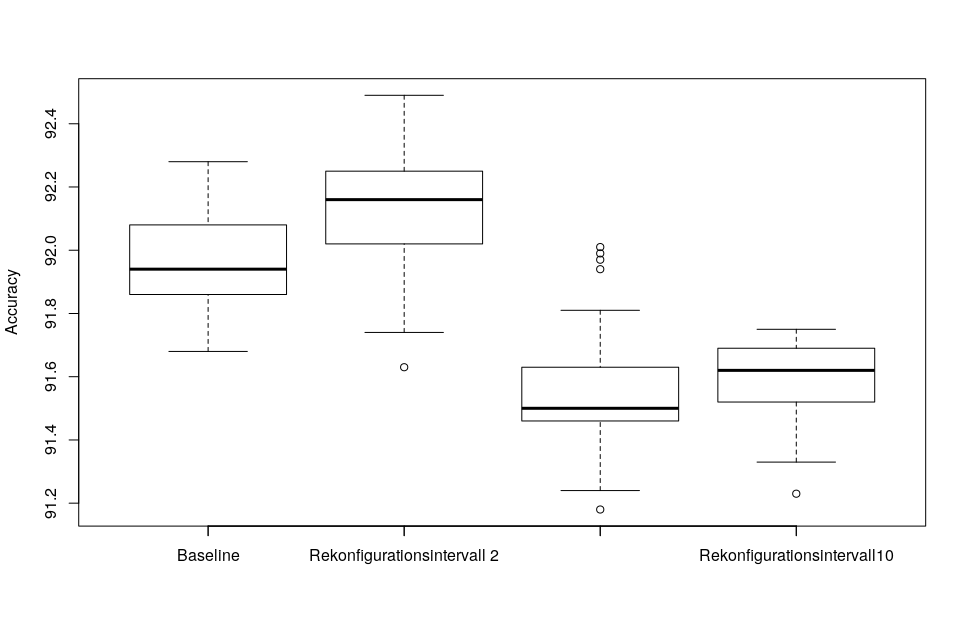
\includegraphics[width=0.47\textwidth]{KapitelPartB/Images/reconf2.png}\label{abb:reconf2}}
 \caption{Boxplot der Rekonfigurationsintervalle}
 \label{abb:reconf}
\end{figure}

 Dies bedeutet, dass der Overhead des Beschneidungsverfahrens geringer ist als der Gewinn durch das Verkleinern des Netzes. In Abbildung \ref{abb:reconf3} ist zu sehen, dass dieser Gewinn an Trainingszeit in Abbildung \ref{abb:reconf2} mit einem Verlust an geringem Verlust an Accuracy einhergeht.  

 
 \begin{figure}[h]
 \centering
 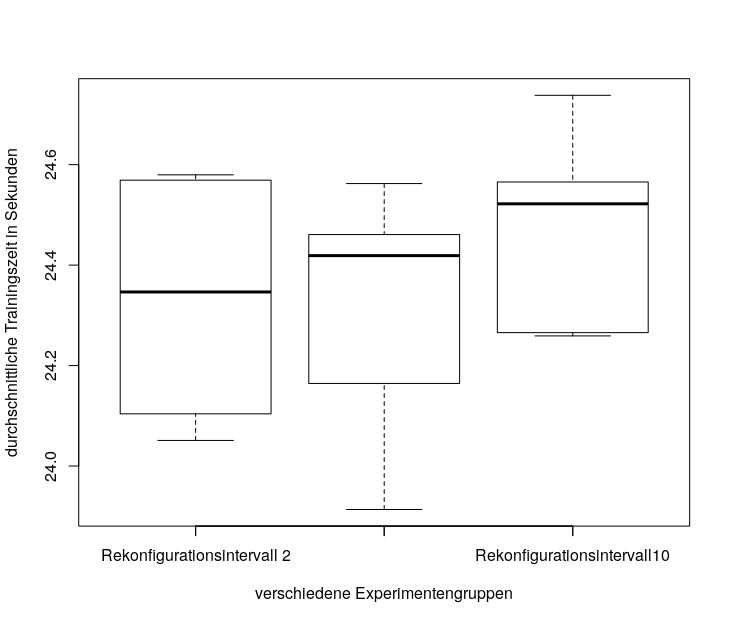
\includegraphics[width=0.5\textwidth]{KapitelPartB/Images/reconf3.png}
 % reconf3.png: 454x491 px, 96dpi, 12.01x12.99 cm, bb=0 0 341 368
 \label{abb:reconf3}
 \caption{Accuracy von verschiedenen Experimentengruppen des Rekonfigurationsintervall}
\end{figure}

 \subsubsection{Experimente zum Grenzwert}


\begin{figure}[h]
 \centering
 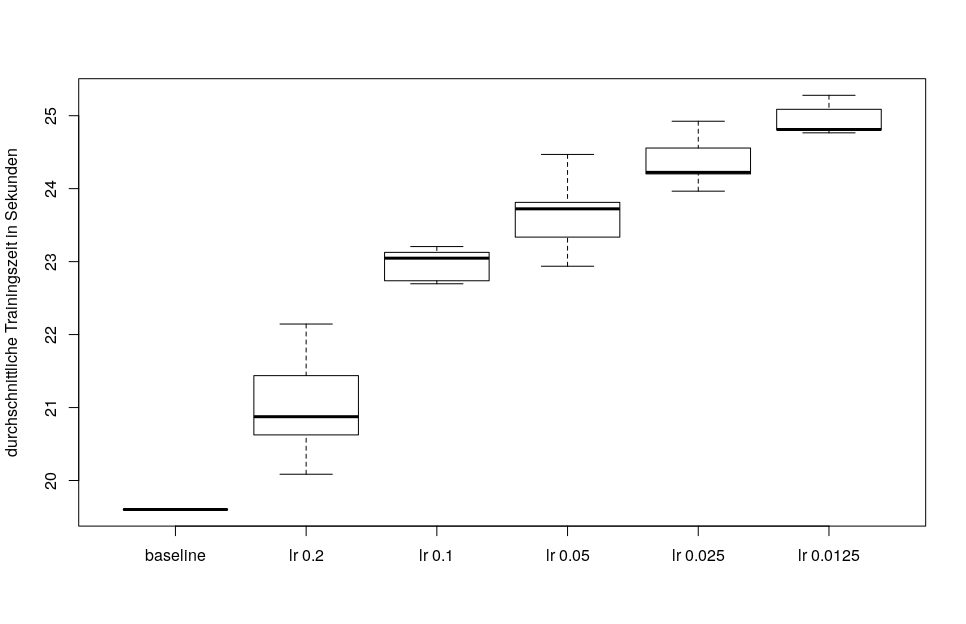
\includegraphics[width=0.8\textwidth]{KapitelPartB/Images/lr1.png}
 % lr1.png: 431x491 px, 96dpi, 11.41x12.99 cm, bb=0 0 323 368
 \label{ref:lra}
\end{figure}

 In Abbildung \ref{abb:lra} ist nicht wirklich was zu sehen, 
 
 
 
Es ergibt sich, dass sich mit diesen bisherigen Experimenten keine Zeit sparen lässt. Im Gegenteil, der PruneTrain Ansatz braucht mehr Zeit. Dies steht im Widerspruch zum PruneTrain Paper. Dieser Widerspruch lässt sich durch die Verwendung von mehreren GPUs zur Evaluation im PruneTrain Paper erklären. Mit einem schmalleren Netz müssen weniger Daten zwischen den GPUs ausgetauscht werden. Es wird Kommunikationszeit gespart.




\todo[inline]{Bis hier muss noch mit mehr Experimenten sichergestellt werden, dass die Effekte nicht an der kleinen Zahl an Experimenten liegt.}
\color{blue1}

\subsubsection{Experimente zur Batchgröße}



Gleichzeitig wird für die jeweilige Modellgrösse die Anzahl an Parametern, die das Modell hat gezählt. Diese Größen sind in Tabelle \ref{tab:batchSize} eingetragen. 


Mit Hilfe dieser Grössen wird für jede einzelne Stagegröße eine Gerade gefittet.

Diese gefittete Gerade wird mittels t-Test darauf überprüft wie wahrscheinlich beim Fitten der Gerade ein Fehler 1. Art auftritt.

Hierfür werden folgende Hypothesen aufgestellt:


Da der p-Wert für diese Gerade bei $p=2,911e^{-16}$ und damit weit unter de Signifikanzniveau von $\alpha=0,05$ kann die $H_0$ Hypothese abgelehnt werden und die Alternativhypothese angenommen werden.

Dies bestätigt statistisch eine hohe Wahrscheinlichkeit, dass die gefittete Gerade richtig ist.



In Abbildung \ref{fig:linearBlocks} ist zu sehen, dass die Parameteranzahl in Zusammenhang mit der Anzahl an Blöcken linear steigt.
Wird das Netz kleiner, so kann anhand der Gerade abhängig von der Parameteranzahl die neue Batchgröße errechnet werden.






\todo{beispielrechnung}

In Abbildung \todo{ref} ist abgebildet. wie sich die Trainingszeiten verändern, wenn die Batchgrösse angepasst wird.



\subsubsection{Veränderung der Accuracy durch PruneTrain}

Durch das Pruning währenddem Training wird die Accuracy kleiner. In Abbildung \ref{abb:PTaccuracy} ist zu sehen wie sich im Accuracy im Verlauf der Epochen verändert.  

\begin{figure}[h]
 \centering
 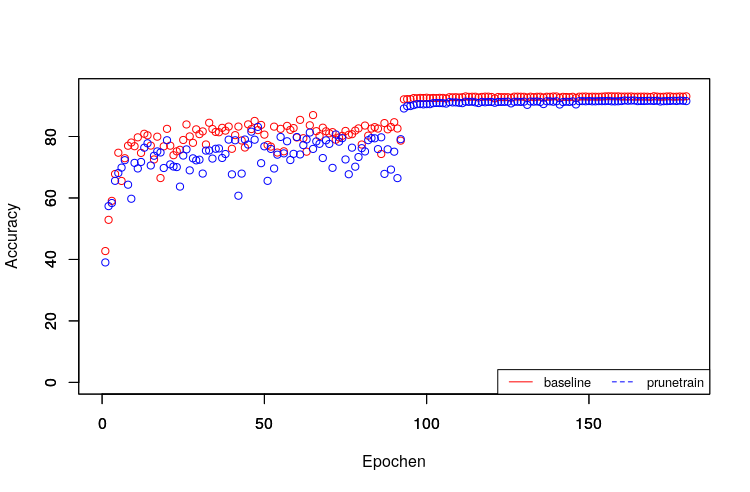
\includegraphics[width=0.8\textwidth]{KapitelPartB/Images/PTaccuracy.png}
 % PTaccuracy.png: 750x492 px, 96dpi, 19.85x13.02 cm, bb=0 0 563 369
 \caption{Veränderung der Accuracy während der Epochen}
 \label{abb:PTaccuracy}
\end{figure}

In Abbildung \ref{abb:PTaccuracyzoom} sind die Epochen 90 bis 180 näher herangezoomt.

\begin{figure}[h]
 \centering
 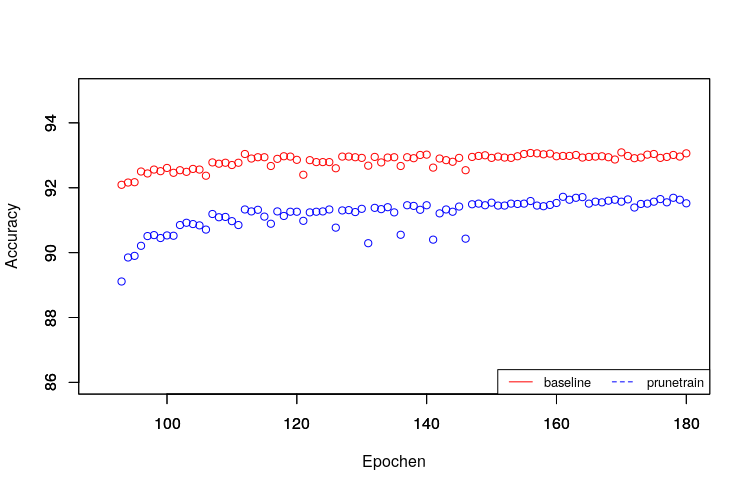
\includegraphics[width=0.8\textwidth]{KapitelPartB/Images/PTaccuracyzoom.png}
 % PTaccuracyzoom.png: 750x492 px, 96dpi, 19.85x13.02 cm, bb=0 0 563 369
 \caption{Zoom der Veränderung}
 \label{abb:PTaccuracyzoom}
\end{figure}

Man sieht eine geringere Accuracy von PruneTrain im Vergleich zum Baseline. Diese Verringerung der Accuracy lässt sich durch ein Aussetzen des Verkleinern des Netzes in den letzten Epochen  
vermindern.

Die Frage die sich hier stellt ist, ob diese Verminderung der Accuracy am Ende der dieser Arbeit noch ins Gewicht fällt. Wenn mit Hilfe einer Kombination von MorphNet und PruneTrain ein bessere Architektur gefunden wird kann diese Architektur auch direkt mit Hilfe des äquivalenten Baseline Netzes berechnet werden.

\subsection{Einfluss der Batchgröße auf PruneTrain}\label{sec:batch}

Das heisst es ist nötig, zu wissen wie gross die Batches maximal sein dürfen um keinen Out of Memory Error zu provozieren. Zusätzlich kann dann berechnet werden, inwieweit die Batchgrösse weiter angehoben werden kann bei kleiner werdendem Netz

Um die Anpassung der Batchgröße an die Verkleinerung des Netzwerkes durch das Prunen zu implmentieren muss zunächst die Batchgröße des Ausgangsnetzes so gewählt werden, dass der GPU-Speicher maximal ausgelastet ist.



Theoretisch sollte hierfür nachdem Übertragen des Modells der freie Speicher ausglesen werden und anhand des Speicherverbrauchs eines Elements des Datensatzes berechnet werden, wie gross die Batchgröße maximal sein darf. Leider führt diese Methode nicht zum gewünschten Ergebnis, da der ausgelesene freie Speicher nicht dem tratsächlich allokierbaren Speicher entspricht.
Der Grund hierfür ist ein Fragmentierungsproblem. Verschiedene freie Blöcke können nicht zu einem grossen allokierbaren Block zusammengefügt werden.\todo[inline]{Quelle}. 

Diese Problem wird mit einer Methode, die für einen beliebigen Datensatz und für eine beliebige Modellgrösse die maximale Batchgröße berechnet, gelöst. 


\todo[inline]{Tabelle mit neuen Zahlen updaten, da mit kaputter Grafikkarte berechnet}
\begin{table}[]
\begin{tabular}{c|c|c|c|c|c|c|c|c|}
\cline{2-9}
                         & \multicolumn{2}{c|}{s=1}  & \multicolumn{2}{c|}{s=2}  & \multicolumn{2}{c|}{s=3}  & \multicolumn{2}{c|}{s=4}  \\ \cline{1-1}
\multicolumn{1}{|l|}{}   & \#Para & Batch & \#Para & Batch & \#Para & Batch & \#Para & Batch \\ \hline
\multicolumn{1}{|l|}{1}  & 7642         & 14272      & 31034        & 5856       & 123898       & 2704       & 493946       & 1344       \\ \hline
\multicolumn{1}{|l|}{2}  & 14650        & 8816       & 65882        & 3328       & 269722       & 1472       & 1082906      & 688        \\ \hline
\multicolumn{1}{|l|}{3}  & 21658        & 6512       & 100730       & 2368       & 415546       & 1024       & 1671866      & 480        \\ \hline
\multicolumn{1}{|l|}{4}  & 28666        & 5072       & 135578       & 1808       & 561370       & 784        & 2260826      & 368        \\ \hline
\multicolumn{1}{|l|}{5}  & 35674        & 4208       & 170426       & 1488       & 707194       & 624        & 2840786      & 288        \\ \hline
\multicolumn{1}{|l|}{6}  & 42682        & 3568       & 205274       & 1232       & 853018       & 528        & 3438746      & 240        \\ \hline
\multicolumn{1}{|l|}{7}  & 49690        & 3120       & 240122       & 1072       & 998842       & 464        & 4027706      & 208        \\ \hline
\multicolumn{1}{|l|}{8}  & 56698        & 2736       & 274970       & 944        & 1144666      & 400        & 4616666      & 176        \\ \hline
\multicolumn{1}{|l|}{9}  & 63706        & 2464       & 309818       & 848        & 1290490      & 352        & 5205626      & 160        \\ \hline
\multicolumn{1}{|l|}{10} & 70714        & 2224       & 344666       & 752        & 1436314      & 320        & 5794586      & 145        \\ \hline
\multicolumn{1}{|l|}{11} & 77722        & 2049       & 379514       & 688        & 1582138      & 288        &              &            \\ \hline
\end{tabular}
\end{table}




\begin{figure}[h]
 \centering
 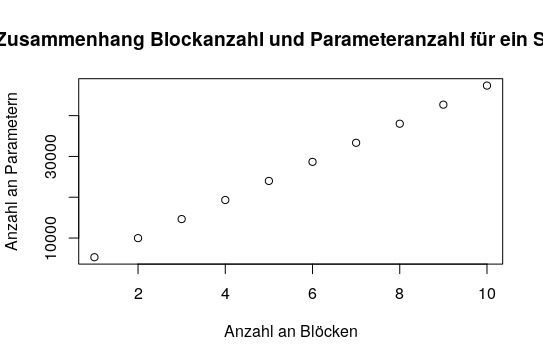
\includegraphics[width=0.8\textwidth]{KapitelPartB/Images/linearBlocks.png}
 % batchSizevsTime.png: 387x367 px, 96dpi, 10.24x9.71 cm, bb=0 0 290 275
 \caption{Batch Size vs Trainings Time über eine Epoche}
 \label{fig:linearBlocks}
\end{figure}




Die maximal mögliche Batchgrösse in Abbildung \ref{fig:maxBatchSize} sinkt im Gegensatz dazu stärker als linear bei mehr Blöcken im Netz. Dies liegt darin begründet, dass für ein grösseres Netz mehr Werte zwischengespeichert werden müssen, was den Speicherbedarf erhöht.

\begin{figure}[h]
 \centering
 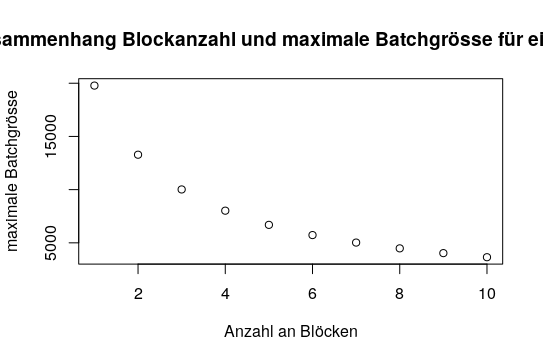
\includegraphics[width=0.8\textwidth]{KapitelPartB/Images/maxBatchSize.png}
 % batchSizevsTime.png: 387x367 px, 96dpi, 10.24x9.71 cm, bb=0 0 290 275
 \caption{Batch Size vs Trainings Time über eine Epoche}
 \label{fig:maxBatchSize}
\end{figure}




Gesucht ist ein idealerweise linearer Zusammenhang zwischen der Parameteranzahl und der Batchgrösse. Um diesen herzustellen wird die Parameteranzahl durch die Batchanzahl geteilt. Das Ergebnis hiervon ist in Abbildung \ref{fig:quotient} zu sehen.

\begin{figure}[h]
 \centering
 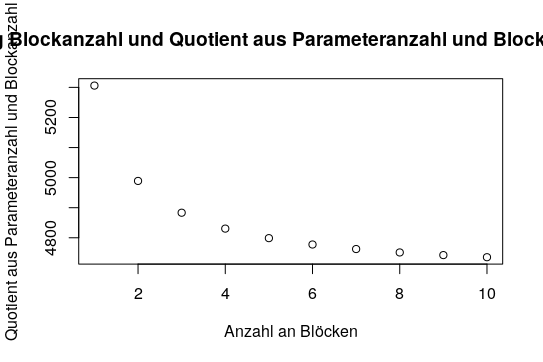
\includegraphics[width=0.8\textwidth]{KapitelPartB/Images/quotient.png}
 % batchSizevsTime.png: 387x367 px, 96dpi, 10.24x9.71 cm, bb=0 0 290 275
 \caption{Batch Size vs Trainings Time über eine Epoche}
 \label{fig:quotient}
\end{figure}


Da diese Kurve ähnlich der Batchsize-Kurve aussieht wird die Hypothese untersucht, ob hier ein linearer Zusammenhang besteht. Zu diesem Zweck wird die Batchgrösse durch das Ergebnis geteilt.

Augenscheinlich liegt hier ein linearer Zusammenhang vor. Daher wird hier eine Gerade gefittet.
Es entsteht die Abbildung \ref{fig:gerade}.

\begin{figure}[h]
 \centering
 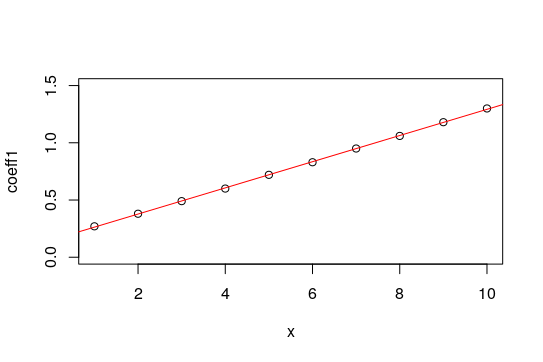
\includegraphics[width=0.8\textwidth]{KapitelPartB/Images/gerade.png}
 % batchSizevsTime.png: 387x367 px, 96dpi, 10.24x9.71 cm, bb=0 0 290 275
 \caption{Batch Size vs Trainings Time über eine Epoche}
 \label{fig:gerade}
\end{figure}




Die gefittete Gerade hat die Gleichung: $$ f(x)=0.11 \cdot x +  0.15 $$

\todo{Hier muss noch das Fitten des Modells und der t-Test erklärt werden}

In Tabelle \todo{Tabelle} werden die Werte für die anderen Stages zusammengefasst. Zu sehen ist, dass für jeden Stage die gefittete Gerade ähnlich im t-Test abschneidet.







Als nächsten Schritt wird untersucht wie das Intervall wie häufig rekonfiguriert wird den Zusammenhang zwischen Inferenz Flop und der Validation Accuracy verändert.


Die nächste Untersuchung über das Sparen von Kommunikationskosten beim Verteilten Training macht hier keinen Sinn da nur eine einzelne Graka genutzt wird.


Abschliessend wird noch evaluiert, wie die Dichte der Gewichte mit der Dichte der Kanäle nachdem Training zusammenhängen um eventuell durch spezifische Inferenzhardware weiter zusparen.





Bei grösserer Batchgrösse wird auch das Netz schneller. Dies ist in Abildung \ref{fig:batchVsTime} für das ResNet und die verwendete Hardware abgebildet.

\begin{figure}[h]
 \centering
 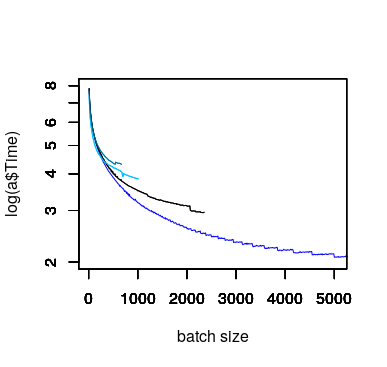
\includegraphics[width=0.8\textwidth]{KapitelPartB/Images/batchSizevsTime.png}
 % batchSizevsTime.png: 387x367 px, 96dpi, 10.24x9.71 cm, bb=0 0 290 275
 \caption{Batch Size vs Trainings Time über eine Epoche}
 \label{fig:batchVsTime}
\end{figure}


Wie zu sehen ist, wird die Trainingszeit pro Epoche mit grösserer Batchgrösse kleiner. Die höhere Batchgrösse sorgt neben der geringeren Trainingszeit auch für weniger Gewichtsupdates. Dies führt zu einer geringeren Generalisationsfähigkeit und damit zu einer geringeren Klassifikationsleistung \cite{largeBatch}. Um diesen Verlust an Klassifikationsleistung auszugleichen gibt es die Möglichkeit die Lernrate anzupassen und eine andere Batch Normalisation zu verwenden \cite{largeBatch}. Diese Technik funktioniert laut dem Paper "`Train longer, generalize better: closing the generalization gap in large batch training of neural networks"' bereits auf residualen Netzen wie sie in dieser Arbeit verwendet werden \cite{largeBatch}. Vorallem bleibt die Einsparung bei der Trainingszeit durch diese Technik intakt \cite{largeBatch}.

Ist dieser Effekt auf PruneTrain übertragbar?


Eine grössere Batchsize sorgt auf jeden Fall für signifikant weniger Verkleinerung des Netzes.
\todo{t-Test um statistisch zu zeigen, dass das signifikant ist}

Die Frage die sich hier stellt ist, ob mit Hilfe von largeBatch bei maximaler Batchsize die Verkleinerungsrate steigt  


\subsubsection{Ghost Batch Norm und LR Anpassung}

\subsubsection{Untersuchung}
Im nächsten Schritt wird untersucht, ob diese Vorteile auch für den PruneTrain Vorgang genutzt werden kann. Dafür wird zunächst untersucht, welchen Effekt eine grössere Batchgrösse auf PruneTrain hat.




Es stellt sich die Frage, ob das einen so grossen Einfluss auf die Ausführungszeit hat.



Man sieht, dass mit steigender Batchgröße die Ausführungszeit sinkt. 

Errechne zusätzlich noch ein Modell, wo abhängig von der Modellgrösse währenddem Pruning die Batchgrösse angepasst wird.



\cite{largeBatch} gibt an, dass mit grösserer Batch size die Accuracy weniger wird. Aber dort wird ein Verfahren angegben, welches diesen Effekt entfernen kann.
Da dieser Effekt da sehr deutlich gezeigt wird hier im nächsten Unterkapitel nur die Überprüfung, ob dieser Effekt auf bei geprunten Netzwerken funktioniert.
\subsection{Einfluss der Batchgrösse und der Lernrate auf die Verkleinerung des Netzes}
\todo[inline,color=blue]{Untersuche, ob largeBatch auch auf ein PruneTrain Netzwerk anwendbar ist.}
\todo[inline,color=brown]{Untersuche, ob die Grösse des Batches beeinflusst, wie viel vom Netz geprunt wird}



\section{Untersuchung von Net2Net}


\section{Untersuchung von MorphNet}

MorphNet macht alle Layer breiter um sie dann mit einem speziellen Regularisierer breiter zu machen. Dieser Regularisierer hat verschiedene mögliche Zielgrössen (Modelgrösse, Flops oder Inferenz-Zeit).
Die Frage stellt sich hier, ob das Netz besser wird wenn alle Schichten breiter gemacht werden um später wieder geprunt zuwerden.

Weiterhin besteht die Möglichkeit das Netz nicht nur breiter zu machen sondern auch tiefer.


MorphNet erwähnt, dass es Sinn macht nicht im ganzen Netz denn Wider Operator anzuwenden sonder nur da wo der Regularisierer das Netz nicht schmaller macht.
\section{PruneTrain + Net2Net}

\section{Additive Verfahren}

\subsection{Zahlenformate}

\begin{itemize}
 \item FP16 bereits probiert
\end{itemize}


FP16 nur auf RTX 2080 sinnvoll
Bietet nach erster Messung etwa 28 \% Prozent Gewinn.

Code für dieses Verfahren liegt vor: Amp apex von Nvidia

AMP bietet 3 mögliche Optimierungsstufen:

O1
Patch all Torch functions and Tensor methods to cast their inputs according to a whitelist-blacklist model. Whitelist ops (for example, Tensor Core-friendly ops like GEMMs and convolutions) are performed in FP16. Blacklist ops that benefit from FP32 precision (for example, softmax) are performed in FP32. O1 also uses dynamic loss scaling, unless overridden.

02
casts the model weights to FP16, patches the models forward method to cast input data to FP16, keeps batchnorms in FP32, maintains FP32 master weights, updates the optimizer’s paramgroups so that the optimizer.step() acts directly on the FP32 weights (followed by FP32 master weight-FP16 model weight copies if necessary), and implements dynamic loss scaling (unless overridden). Unlike O1, O2 does not patch Torch functions or Tensor methods.


O3
may not achieve the stability of the true mixed precision options O1 and O2. However, it can be useful to establish a speed baseline for your model, against which the performance of O1 and O2 can be compared. If your model uses batch normalization, to establish speed of light you can try O3 with the additional property override keepBatchnormfp32=True (which enables cudnn batchnorm, as stated earlier).

Hier nur O0, O1 und O2 dargestellt, da O3 absolut nicht mithalten kann was Performance angeht.

\begin{figure}[h]
 \centering
 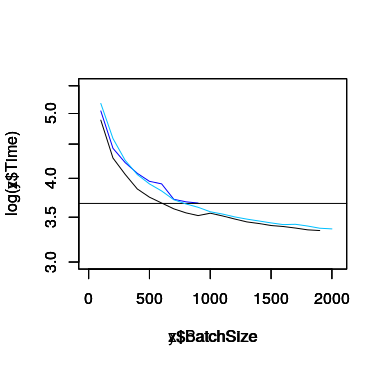
\includegraphics[width=0.8\textwidth]{KapitelPartB/Images/timeVsBatchSize_Amp.png}
 % timeVsBatchSize_Amp.png: 387x367 px, 96dpi, 10.24x9.71 cm, bb=0 0 290 275
 \caption{Vergleich Trainingszeit einer Epoche für verschiedene Optimierungsstufen von Amp Apex. DunkelBlau=O0; Schwarz = O1; Hellblau=O2}
 \label{fig:amp}
\end{figure}

\todo[inline,color=brown]{Weitere Versuche, die zeigen ob die Zeiten grossen statistischen Schwankungen unterliegen.}
\url{https://developer.download.nvidia.com/video/gputechconf/gtc/2019/presentation/s9998-automatic-mixed-precision-in-pytorch.pdf} zeigt, dass bezüglich der Accuracy kein Verlust zu erwarten ist.

Da O2 gegenüber O1 keinen signifikanten zusätzlichen Gewinn bringt nutze O1.
\subsection{Beschleunigung der Berechnung des Gradientenabstiegverfahren}


Accelerating CNN Training by Sparsifying Activation Gradients funktioniert nur auf Toy-Benchmarks 


\subsubsection{Weight Normalization: A Simple Reparameterization
to Accelerate Training of Deep Neural Networks}

\todo[inline,color=blue]{Testen ob es funktioniert}
Könnte funktionieren. Code für Lasagne: https://github.com/TimSalimans/weight\_norm


\subsubsection{Accelerating Deep Neural Network Training with Inconsistent Stochastic Gradient Descent}

Interessant bisher kein Code verfügbar
\todo[inline, color=blue]{Implementieren (ist einfach) und testen}

\subsubsection{Accelerated CNN Training Through Gradient Approximation }

Interessant bisher kein Code verfügbar





\chapter{Ausblick und Fazit}\label{sec:fazit}
Es hat sich gezeigt, dass MorphNet den Nachteil hat, dass die Tiefe des Netzes nicht verändert werden kann. Diesen Nachteil kann Net2Net als potentieller Kandidat einer erweiternden Methode einer Kombination ausgleichen. Es zeigt sich bei allen Verfahren, dass eine Anpassung der Lernrate Sinn macht. 

Es wäre sowohl für MorphNet als auch für die Kombination ein potentieller Gewinn, wenn die Lernrate automatisch angepasst werden würde, bevor eine Anpassung der Struktur passiert. Der Grund, wieso dies sinnvoll ist liegt daran, dass ohne Anpassung der Lernrate nicht das volle Potential jedes Modells genutzt werden kann. Hier wäre es allerdings notwendig nach der Veränderung der Struktur zu evaluieren, wie mit der Lernrate weiter zu verfahren ist. Die Anpassung der Lernrate sollte hier sowohl bei einem Plateau in der Accuracy als auch bei nicht stabilen Training funktionieren.


Da sich beim Training der verschiedenen Netze gezeigt hat, dass diese unterschiedlich lange brauchen, um ihr Potential auszuschöpfen ist es sinnvoll die Epoche zu der ein Operator von Net2Net angewendet wird flexibel anhand des Accuracy Verlaufs zu gestalten.  


Die Erkundung des Modellraumes zeigt, dass sich Net2Net auch bei kleinen Ausgangsnetzen lohnt. Für die Kombination wäre es hilfreich, mit Hilfe der Ergebnisse des Beschneidens zu entscheiden welcher Operator angewendet wird. 

Bei den verschiedenen Verfahren ist zu beobachten, dass in allen vorgestellten Fällen ein Trade-off zwischen Accuracy und Trainingszeit zu beobachten ist.


% Anhang ---------------------------------------------------------------
%
\cleardoublepage
\appendix

%========================================================================================
% TU Dortmund, Computer Science VII
%========================================================================================
\chapter{d}


%
\listoffigures
\addcontentsline{toc}{chapter}{Abbildungsverzeichnis}
\cleardoublepage


\cleardoublepage

%
\addcontentsline{toc}{chapter}{Literaturverzeichnis}
\bibliographystyle{alpha}
\bibliography{Literature}

% ----------------------------------------------------------------------

\end{document}
